%!TeX spellcheck=en_US
\documentclass[11pt,
               a4paper,
               bibtotoc,
               idxtotoc,
               headsepline,
               footsepline,
               footexclude,
               BCOR12mm,
               DIV13,
               openany,   % using this removes blank pages around part / chapter starts.
%               oneside    % include this if you have to print only one page per sheet of paper.
               ]
               {scrbook}

\input{settings}
\newglossaryentry{cog}{name=COG, description={Center of Gravity Defuzzification Method}}
\newglossaryentry{som}{name=SOM, description={Start of Maximum Defuzzification Method}}
\newglossaryentry{mom}{name=MOM, description={Mean of Maximum Defuzzification Method}}
\newglossaryentry{fcs}{name=FCS, description={Fuzzy Control System}}
\newglossaryentry{autopas}{name=AutoPas, description={Node-level auto-tuned particle simulation library written in C++. See \url{https://github.com/AutoPas/AutoPas}}}
\newglossaryentry{mdflexible}{name=md\_flexible, description={A flexible molecular dynamics simulation framework built on top of \gls{autopas}}}

\usepackage{lipsum} % for filling pages with stuff
\usepackage{todonotes} % for todo notes

\setlipsum{auto-lang=false} % to avoid babel errors


\includeonly{
    content/3Implementation,
}

% -------------------------------------------------------------------------------
% --------------------------------- Thesis Info ---------------------------------
% -------------------------------------------------------------------------------

% set title, authors and stuff for the cover
% docytype needs xspace because it is used within text.
\def\doctype{Bachelor's Thesis\xspace}
%\def\doctype{Master's Thesis\xspace}
%\def\doctype{Guided Research\xspace}
%\def\doctype{Interdisciplinary Project\xspace}
\def\studyProgram{Informatics}
\def\title{Exploring Fuzzy Tuning Technique for Molecular Dynamics Simulations in AutoPas}
% don't try translate every technical term if it would sound off
\def\titleGer{Untersuchung von Fuzzy Tuning Verfahren für Molekulardynamik-Simulationen in AutoPas}
\def\author{Manuel Lerchner}
% Prof
\def\supervisor{Univ.-Prof. Dr. Hans-Joachim Bungartz}
% PhD Candidate
\def\advisorFst{Manish Kumar Mishra, M.Sc.}
\def\advisorSnd{Samuel Newcome, M.Sc.}
\def\date{10.08.2024}
\begin{document}
\frontmatter
% -------------------------------------------------------------------------------
% ---------------------------------- COVERPAGE ----------------------------------
% -------------------------------------------------------------------------------

% correct BCOR - undo at the end !!!
\def\bcorcor{0.15cm}
\addtolength{\hoffset}{\bcorcor}
\thispagestyle{empty}
\vspace{4cm}
\begin{center}
    \includegraphics[width=4cm]{templateStuff/tumlogo.pdf}\\[5mm]
    \huge SCHOOL OF COMPUTATION, INFORMATION AND TECHNOLOGY\\[5mm]
    \large DER TECHNISCHEN UNIVERSITÄT MÜNCHEN\\[24mm]

    {\Large \doctype in \studyProgram}\\[20mm]
    {\huge\textbf{\title}\par}
    \vspace{15mm}
    {\LARGE  \author}
\end{center}

\cleardoubleemptypage

% -------------------------------------------------------------------------------
% ---------------------------------- TITLEPAGE ----------------------------------
% -------------------------------------------------------------------------------

\def\bcorcor{0.15cm}
\addtolength{\hoffset}{\bcorcor}
\thispagestyle{empty}
\vspace{10mm}
\begin{center}
    \includegraphics[width=4cm]{templateStuff/tumlogo.pdf}\\[5mm]
    \huge SCHOOL OF COMPUTATION, INFORMATION AND TECHNOLOGY\\[5mm]
    \large DER TECHNISCHEN UNIVERSITÄT MÜNCHEN\\[24mm]
    {\Large \doctype in \studyProgram}\\[20mm]
    \todo{Remove all TODOS}  {\LARGE\textbf{\title}}\\[10mm]
    {\LARGE\textbf{\titleGer}}\\[10mm]
    \begin{tabular}{ll}
        \Large Author:     & \Large \author                     \\[2mm]
        \Large Supervisor: & \Large \supervisor                 \\[2mm]
        \Large Advisors:   & \Large \advisorFst \nobreakspace\& \\[2mm]
        \Large             & \Large \advisorSnd                 \\[2mm]
        \Large Date:       & \Large \date
    \end{tabular}

\end{center}

% undo BCOR correction
\addtolength{\hoffset}{\bcorcor}
\newpage

% -------------------------------------------------------------------------------
% ---------------------------------- DISCLAIMER ---------------------------------
% -------------------------------------------------------------------------------

\cleardoubleemptypage

\thispagestyle{empty}
\vspace*{0.7\textheight}
\noindent
I confirm that this \MakeLowercase{\doctype} is my own work and I have documented all sources and material used.\\

\vspace{15mm}
\noindent
Munich, \date \hspace{5cm} \author
\cleardoubleemptypage

% -------------------------------------------------------------------------------
% ------------------------------- ACKNOWLEDGEMENTS ------------------------------
% -------------------------------------------------------------------------------

\phantomsection
\addcontentsline{toc}{chapter}{Acknowledgements}
\vspace*{2cm}
\begin{center}
    {\Large \textbf{Acknowledgements}}
\end{center}
\vspace{1cm}

\lipsum[1]

\cleardoublepage

% -------------------------------------------------------------------------------
% ---------------------------------- ABSTRACT -----------------------------------
% -------------------------------------------------------------------------------

\phantomsection
\addcontentsline{toc}{chapter}{Abstract}
\vspace*{2cm}
\begin{center}
    {\Large \textbf{Abstract}}
\end{center}
\vspace{1cm}

AutoPas is a high-performance, auto-tuned particle simulation library for many-body systems, capable of dynamically switching between algorithms and data structures based on their performance in the current simulation state.
This thesis introduces a novel fuzzy logic-based tuning strategy for AutoPas, allowing users to guide tuning phases by specifying custom Fuzzy Systems, which can be used to efficiently prune the search space of possible parameter configurations. Efficient tuning strategies are crucial, as they allow for discarding poor parameter configurations without evaluating them, thus reducing tuning time and improving overall library performance.

We demonstrate that a data-driven approach can automatically generate Fuzzy Systems that significantly outperform existing tuning strategies on specific benchmarks. The proposed Fuzzy Tuning Strategy achieves speedups of up to 1.96x compared to the FullSearch Strategy on scenarios included in the training data and up to 1.35x on scenarios not directly included.

The Fuzzy Tuning Strategy can drastically reduce the number of evaluated configurations during tuning phases while achieving comparable tuning results, making it a viable alternative to the existing tuning strategies.

\cleardoublepage

\phantomsection
\addcontentsline{toc}{chapter}{Zusammenfassung}
\vspace*{2cm}
\begin{center}
    {\Large \textbf{Zusammenfassung}}
\end{center}
\vspace{1cm}

AutoPas ist eine hochperformante, selbstoptimierende Teilchensimulationsbibliothek für Mehrkörpersysteme, welche in der Lage ist, dynamisch zwischen verschiedenen Algorithmen und Datenstrukturen zu wechseln und diese entsprechend ihrer Leistung im aktuellen Simulationszustand anzupassen.
In dieser Arbeit wird eine neuartige, auf Fuzzy-Logik basierende Tuning-Strategie für AutoPas vorgestellt, die es dem Benutzer ermöglicht, Tuning-Phasen durch die Vorgabe von benutzerdefinierten Fuzzy-Systemen zu steuern, um so den Suchraum möglicher Parameterkonfigurationen effizient zu verkleinern. Solche effizienten Suchstrategien sind von entscheidender Bedeutung für AutoPas, da sie den Ausschluss ungünstiger Parameter-Konfigurationen ermöglichen, ohne diese zu evaluieren.

Wir zeigen, dass ein datengetriebener Ansatz zur automatischen Generierung von Fuzzy-Systemen in bestimmten Tests eine deutlich bessere Leistung als bestehende Tuning-Strategien erbringen kann. Die vorgeschlagene Fuzzy- Tuning-Strategie erreicht eine bis zu 1,96-fache Leistungssteigerung im Vergleich zur FullSearch-Strategie für Szenarien, die in den Trainingsdaten enthalten sind, und eine bis zu 1,35-fache Steigerung für Szenarien, die nicht unmittelbar in den Trainingsdaten enthalten sind.

Die Fuzzy-Tuning-Strategie kann die Anzahl der evaluierten Konfigurationen während der Tuning-Phasen drastisch reduzieren, während sie vergleichbare Tuning-Ergebnisse erzielt, wodurch sie eine vielversprechende Alternative zu den bestehenden Tuning-Strategien darstellt.


\cleardoublepage

% -------------------------------------------------------------------------------
% ------------------------------ TABLE OF CONTENTS ------------------------------
% -------------------------------------------------------------------------------

\tableofcontents
\thispagestyle{empty}
\cleardoubleemptypage

% -------------------------------------------------------------------------------
% --------------------------------- MAIN MATTER ---------------------------------
% -------------------------------------------------------------------------------

\mainmatter

\chapter{Introduction}
\label{sec:intro}
Write some useful intro. Here are tips along the way:

\section{A}
\chapter{Theoretical Background}
\label{sec:theoretical_background}


\section{Molecular Dynamics}

Molecular Dynamics (MD) is a computational method used to simulate the behavior of atoms and molecules over time. In recent years, MD simulations have become essential in many scientific fields, including chemistry, physics, biology, and materials science. MD simulations are used to study various systems, ranging from simple gases and liquids to complex biological molecules and materials.

MD simulations' main goal is to understand complex systems' behavior at an atomic level and to predict their properties and behavior under different conditions. Using the power of computer simulations, where fundamental properties of the experiment can be changed by adjusting some formulas and parameters, allows researchers to study a wide variety of systems and conditions at a level of detail that is inaccessible to experimental methods alone~\cite{Perilla2017}.

Two examples of such simulations are shown in \autoref{fig:hiv_capsid} and \autoref{fig:md_simulation_loop}. The first image shows a simulation of the HIV-1 capsid, a protein shell that surrounds the genetic material of the human immunodeficiency virus (HIV). The second image shows an application of MD simulations in materials science, where researchers used computer simulations to study the crack formation in metallic glass.


\begin{multicols*}{2}
      \begin{figure}[H]
            \centering
            \includegraphics[width=1\columnwidth, trim={0cm 0 0cm 0cm}]{figures/Intro/HIV-1.png}
            \caption{Molecular dynamics simulations of the HIV-1 capsid. Perilla et al.~\cite{Perilla2017} used a simulation containing 64,423,983 atoms to investigate different properties of the HIV-1 capsid at an atomic resolution.}
            \label{fig:hiv_capsid}
      \end{figure}

      \begin{figure}[H]
            \centering
            \includegraphics[width=0.9\columnwidth,trim={0cm 0 0cm 0cm}]{figures/Intro/metallic-glass-crack.jpg}
            \caption{Molecular dynamics simulations of shear band formation around a precipitate in metallic glass, as demonstrated by Brink et al.~\cite{Brink2016}.}
            \label{fig:md_simulation_loop}
      \end{figure}
\end{multicols*}

\subsection{Quantum Mechanics and the Schrödinger Equation}

Our current knowledge of physics suggests that the behavior of atoms and molecules is governed by the laws of quantum mechanics, where particles are described by wave functions and probabilities evolving. The physicist Erwin Schrödinger first formulated a mathematical model describing this phenomenon in 1926, which has gotten widespread acceptance and is now known widely as the Schrödinger equation. The Schrödinger equation is a partial differential equation describing how a physical system's wave function evolves over time. It is typically written as:

\begin{equation}
      i \hbar \frac{\partial \Psi}{\partial t} = \hat{H} \Psi
\end{equation}

Where $\Psi$ is the system's wave function, $\hat{H}$ is the Hamiltonian operator describing the system's energy, $t$ is the time, and $\hbar$ is the reduced Planck constant.

The Schrödinger equation provides a way to calculate the future states of a quantum system given the current state of the system. However, solving the Schrödinger equation for systems with many particles is computationally very expensive and quickly becomes infeasible for systems with more than a few particles~\cite{Leimkuhler2015}. Simulating a single water molecule consisting of three nuclei and 10 electrons would require solving a partial differential equation with 39 variables (The molecule consists of two hydrogen atoms, one oxygen atom, and 10 electrons. Each of those 13 objects is described by three spatial coordinates). Consequently, the resulting Shcrödinger equation also includes all 39 variables and looks like this:

\begin{equation}
      i \hbar \frac{\partial \Psi}{\partial t} = -\hbar^2 \sum_{i=1}^{13} \frac{1}{2m_i} \left( \frac{\partial^2 \Psi}{\partial x_i^2} + \frac{\partial^2 \Psi}{\partial y_i^2} + \frac{\partial^2 \Psi}{\partial z_i^2} \right) + U_p (x_1, y_1, z_1, \ldots, x_{13}, y_{13}, z_{13}) \Psi
\end{equation}

Where $m_i$ is the mass of the $i$-th object, $x_i$, $y_i$, and $z_i$ are the spatial coordinates of the $i$-th object, and $U_p$ is the potential energy function of the system.

As the Schrödinger equation is a partial differential equation, it is computationally expensive to solve for systems with many particles, as one quickly runs into the curse of dimensionality.

The Born-Oppenheimer approximation simplifies this problem by exploiting the significant mass difference between electrons and nuclei. From the perspective of fast-moving electrons, the much heavier nuclei appear nearly stationary, which justifies the separation of electronic and nuclear motions, treating the nuclei as classical particles. The electronic degrees of freedom can then be integrated out, deriving a new energy function $U$ that depends solely on nuclear positions.
This potential energy surface $U$ is typically obtained through quantum mechanical calculations or fitted to empirical data.

However, this approach is still just an approximation, and depending on the chosen potential energy function U, the Born-Oppenheimer approximation may neglect certain quantum mechanical effects, causing inaccuracies in the simulation results.


Despite these limitations, the Born-Oppenheimer approximation is widely used in molecular dynamics simulations as it allows for the simulation of systems with many particles in the first place.

After applying the Born-Oppenheimer approximation and using Newton's second law of motion, the Schrödinger equation can be transformed into a system of ordinary differential equations. Each of those equations describes the motion of a single particle and is given by:

\begin{align}
      m_i \frac{d^2 x_i}{dt^2} & = -\frac{\partial U}{\partial x_i} \\
      m_i \frac{d^2 y_i}{dt^2} & = -\frac{\partial U}{\partial y_i} \\
      m_i \frac{d^2 z_i}{dt^2} & = -\frac{\partial U}{\partial z_i}
\end{align}

Where $m_i$ is the mass of the $i$-th particle, $x_i$, $y_i$, and $z_i$ are the spatial coordinates of the $i$-th particle, and $U$ is the newly derived potential energy function of the system.

\subsection{Numerical Integration}

Since the simulation domain potentially consists of a vast number of particles all interacting with each other, it is generally not possible to solve the equations of motion analytically. This problem is known under the N-body problem, and it can be shown that there are no general solutions for systems with more than two particles. We can, however, solve the equations of motion numerically using numerical integration methods. A standard method to solve the equations of motion numerically is the Verlet algorithm. This integration scheme is derived from the Taylor expansion of the position of the $i$-th object $\vec{r}_i$ at time $t - \Delta t$ and $t + \Delta t$ and is given by:

\begin{equation}
      \vec{r}_i(t + \Delta t) = 2 \vec{r}_i(t) - \vec{r}_i(t - \Delta t) + \vec{a}_i(t) \Delta t^2
\end{equation}

Where $\vec{a}_i(t)$ is the acceleration of the $i$-th object at time $t$ and can be calculated from the particle mass and the acting forces using Newton's second law of motion $\vec{a}_i(t) =\frac{F_i}{m_i}= \frac{-\nabla_i U}{m_i}$.

\subsection{Potential Energy Function}

As stated above, the potential energy function $U$ is a critical component of the molecular dynamics simulation as it fundamentally defines the properties of the system. MD simulations use many different potential energy functions, all of which are tailored to describe specific aspects of the system. Those potentials typically use a mixture of 2-body, 3-body, and 4-body interactions between the particles. The 2-body interactions express the effect of Pauli repulsion, atomic bonds, and coulomb interactions, while higher-order interactions allow for potentially asymmetric wave functions~\cite{Leimkuhler2015}.

A common choice for the potential energy function is the Lennard-Jones potential. The simplicity of the Lennard-Jones potential makes it a popular choice for many systems, as it can be computed efficiently and still captures the attractive and repulsive forces between particles quite well. The Lennard-Jones potential is given by:

\begin{equation}
      U_{LJ}(r) = 4 \epsilon \left[ \left( \frac{\sigma}{r} \right)^{12} - \left( \frac{\sigma}{r} \right)^6 \right]
\end{equation}


Where $r$ is the distance between the particles, $\epsilon$ is the depth of the potential well, and $\sigma$ is the distance at which the potential is zero.

\subsection{Simulation Loop}

Using the methods described above, it is possible to simulate the behavior of a system of particles over time. The general simulation loop for a molecular dynamics simulation can be described as follows:

\begin{enumerate}
      \item \textbf{Initialization} \\
            The simulation starts by initializing the positions and velocities of the particles. The initial positions and velocities can be chosen randomly or based on experimental data.

      \item \textbf{Position Updates} \\
            In this step, the positions of the particles are updated using a numerical integration scheme such as the Verlet algorithm.

      \item \textbf{Force Calculation} \\
            The forces acting on the particles are calculated based on the current positions of the particles and the chosen potential energy function $U$.

      \item \textbf{Update Velocities and Accelerations} \\
            The acceleration of each particle is calculated using Newton's second law of motion. The velocities of the particles are then updated using the acceleration and the time step $\Delta t$.

      \item \textbf{Apply External Forces or Constraints} \\
            In this step, the simulation can be modified by applying external forces or constraints to the particles. In this stage, it is possible to introduce boundary conditions, temperature control, or other outside effects to the simulation.

      \item \textbf{Update Time and Repeat} \\
            The simulation time is updated by advancing it by the time step $\Delta t$. The simulation loop returns to step 2 and repeats until the desired number of integration steps is reached.
\end{enumerate}


Many different software packages exist to perform such simulations. Some widely used examples of such systems are LAAMPS\footnote{\url{https://lammps.sandia.gov/}} and GROMACS\footnote{\url{https://www.gromacs.org/}}. Both efficiently solve the underlying N-body problem and provide the user with a high-level interface to specify the simulation parameters.

Many different approaches exist to efficiently solve the N-body problem, and no single best approach works well for all systems as the optimal implementation heavily depends on the simulation state and the hardware's capabilities to perform the simulation. However, LAAMPS and GROMACS use a single implementation and cannot adapt their algorithms to the current simulation state.

In the following section, we will introduce AutoPas, a library designed to efficiently deal with changing simulation states and capable of automatically adapting to the current simulation state to achieve optimal performance.

\section{AutoPas}

AutoPas is an open-source library designed to achieve optimal performance at the node level for short-range particle simulations. On a high level, AutoPas can be seen as a black box performing arbitrary N-body simulations with short-range particle interactions. The main goal of AutoPas is to provide a high-level interface for the user to perform simulations without worrying about the low-level details of the simulation. This is achieved by providing a high-level interface for the user to interact with the library while the library itself takes care of the low-level details of the force calculations

AutoPas provides many different algorithmic implementations for the problem of N-body simulations, each with different performance and memory usage trade-offs. No single implementation is optimal for all simulation scenarios \todo{find reference}, as the optimal implementation depends on the current simulation state.
AutoPas is designed to be adaptive and can periodically switch between different implementations to achieve the best performance for the current simulation state. This is achieved by allowing AutoPas to automatically tune its internal parameters to find the best implementation for the current simulation state.


Since AutoPas provides a high-level interface for short-range N-body simulations, the user specifies the acting forces between the particles and controls the simulation loop. Fortunately, AutoPas also provides \texttt{\gls{mdflexible}}, an example of a typical molecular dynamics simulation implementation.

\subsection{Autotuning in AutoPas}

AutoPas internally alternates between two phases of operation. The first phase is the \emph{tuning phase}, where AutoPas tries to find the best configuration of parameters about a chosen performance metric. This optimal configuration is then used in the following \emph{simulation phase}, assuming that the optimal configuration found in the tuning phase still performs reasonably well during the consequent simulation phase. As the simulation progresses and the characteristics of the system change, the previously chosen configuration can drift arbitrarily far from the actual optimal configuration. To counteract this, AutoPas periodically alternates between tuning and simulation phases to ensure that the used configuration is reasonably close to the optimal configuration.
AutoPas acts as a black box during the simulation phase, solving the force calculations for the underlying N-body problem.


The power of AutoPas comes from its vast amount of tunable parameters and enormous search space. As mentioned, their design limits other software packages like LAAMPS and GROMACS to just one implementation. They can, therefore, operate outside of the theoretical
optimal performance regime. In the following section, we will discuss the tunable parameters in AutoPas and the different tuning strategies available to find the best configuration of parameters for the current simulation state.


\subsection*{Tunable Parameters}

AutoPas currently provides six tunable parameters, which can mostly\footnote{There are some exceptions as some choices of parameters are incompatible with each other.} be combined freely. A collection of parameters is called a \emph{Configuration}, and the set of all possible configurations is called the \emph{Search Space}. A configuration consists of the following parameters:

\begin{enumerate}[label=\textbf{\arabic*.}]
      \item \textbf{Container Options:} \\
            The container options are related to the data structure used to store the particles. The most important categories of data structures in this section are:
            \begin{enumerate}
                  \item \textbf{DirectSum} \\
                        DirectSum does not use any additional data structures to store the particles. Instead, it simply holds a list of all particles and performs a brute-force calculation of the forces between all pairs of particles. This results in a complexity of $O(N^2)$ distance checks in each iteration. This method is simple and does not require additional data structures, but it has an inferior complexity, making it unsuitable for larger simulations. \textit{Generally should not be used except for tiny systems or demonstration purposes.~\cite{VICCIONE2008625}}
                  \item \textbf{LinkedCells} \\
                        LinkedCells segments the domain into a regular cell grid and only considers interactions between particles from neighboring cells. This results in the trade-off that particles further away than the cutoff radius are not considered for the force calculation. This is not a big issue in practice, as all short-range forces drop off quickly with distance anyway. Additionally, LinkedCells provides a high cache hit rate as particles inside the same cell can be stored contiguously in memory. Typically, the cell size is chosen to be equal to the cutoff radius $r_c$, meaning that each particle only needs to check the forces with particles inside the $3\times3\times3$ cell grid around it as all other particles are guaranteed to be further away than the cutoff radius. This reduction in possible interactions can result in a complexity of just $O(N)$ distance checks in each iteration. However, there is still room for improvement as constant factors can be pretty high. This is especially obvious, as most distance checks performed by LinkedCells still do not contribute to the force calculation~\cite{GRATL2019748}. This trend can be explained due to the uneven scaling of sphere and cube volumes, especially for higher dimensions. For example, in 3D, the ratio of the volume of a sphere with radius $r_c$ to the volume of a cube with side length $3r_c$ is given by:

                        \begin{equation}
                              \frac{\text{Interaction Volume}}{\text{Search Volume}} =
                              \frac{V_{sphere}(r_c)}{V_{cube}(3r_c)} = \frac{\frac{4}{3}\pi r_c^3}{(3r_c)^3} = \frac{4}{81}\pi \approx 0.155
                        \end{equation}

                        This means that only about 15.5\% of all particles present in the $3\times3\times3$ cell grid around a particle are within the cutoff radius.

                        \textit{However, still generally good for large, homogeneous\footnote{Homogeneous in this context, the particles are distributed evenly across the domain.} systems.}

                  \item \textbf{VerletLists} \\
                        VerletLists is another approach to creating neighbor lists for the particles. Contrary to LinkedCells, VerletLists does not rely on a regular grid but instead uses a spherical region around each particle to determine its relevant neighbors.
                        The algorithm creates and maintains a list of all particles present in a sphere within radius $r_c \cdot s$ around each particle, where $r_c$ is the cutoff radius and $s>1$ is the skin factor allowing for a buffer zone around the cutoff radius.
                        By choosing a suitable buffer zone, such that no fast-moving particle can enter the cutoff radius unnoticed, it is possible to only recalculate the neighbor list every few iterations. This approach can benefit systems with high particle density and frequent interactions, as the neighbor list only needs to be updated every $n$ iteration. This results in a complexity of $O(N)$ distance checks in each iteration.
                        We can repeate the calculation from above to determine the ratio of the interaction volume to the search volume for VerletLists:

                        \begin{equation}
                              \frac{\text{Interaction Volume}}{\text{Search Volume}} =
                              \frac{V_{sphere}(r_c)}{V_{sphere}(r_c \cdot s)} = \frac{\frac{4}{3}\pi r_c^3}{\frac{4}{3}\pi (r_c \cdot s)^3} = \frac{1}{s^3}
                        \end{equation}

                        The ratio can be adjusted by changing the skin factor $s$ this time.         Ideally, the skin factor should be chosen so the ratio is close to 1. However, this reduces the buffer zone around the cutoff radius, meaning that the neighbor list needs to be updated more frequently. We conclude that choosing a skin factor that is too small can result in particles entering the cutoff radius unnoticed, leading to incorrect results, while choosing a skin factor that is too large can result in unnecessary distance checks.

                        Compared to LinkedCells, VerletLists can be constructed so that there are few unnecessary distance checks. However, constructing the neighbor list is quite memory intensive and can result in a high memory overhead. Additionally, the neighbor list needs to be updated every few iterations, which can result in a performance overhead.

                        \textit{Generally good for large systems with high particle density.}

                  \item \textbf{VerletClusterLists} \\
                        VerletClusterLists differ from regular VerletLists in the way the neighbor lists are stored. Instead of storing the neighbor list for each particle separately, $n_{cluster}$ particles are grouped into a so-called \emph{cluster}, and a single neighbor list is created for each cluster. This reduces memory overhead as the neighbor list only needs to be stored once for each cluster. Whenever two clusters are close, all interactions between the particles in the two clusters are calculated. This also results in a complexity of $O(N)$ distance checks in each iteration.

                        The main advantage of VerletClusterLists is the reduced memory overhead compared to regular VerletLists. However, constructing the neighbor list is still quite memory intensive and can result in a high memory overhead.

                        \textit{Generally suitable for large systems with high particle density}

            \end{enumerate}

      \item \textbf{Load Estimator Options:} \\
            The Load Estimator Options are related to the way the simulation is parallelized. The load estimator is responsible for estimating the computational load of each MPI rank and how the work is distributed among the ranks. In this thesis, however, we will not further detail the Load Estimator Options as we primarily focus on the tuning aspect of single-node simulations.

      \item \textbf{Traversal Options:} \\
            These options are related to the traversal algorithm used to calculate the forces between the particles. The traversal determines the order in which the particles are visited and how the forces are calculated.
            The different traversal options efficiently prevent race conditions when using multiple threads and allow load balancing at the node level ~\cite{SECKLER2021101296}.

            Many different traversal algorithms are available in AutoPas, each with different performance and optimization potential trade-offs. In the following, we will discuss the most interesting traversal categories:

            \begin{enumerate}

                  \item \textbf{Colored Traversal} \\
                        Since both LinkedCells and VerletLists only consider interactions with particles from neighboring cells/particles, it is possible to parallelize the force calculation by calculating forces for particles in different cells in parallel. This is, however, only possible if all simultaneously calculated particles do not share familiar neighbors, as this would introduce data races when updating the forces of the particles. This is where the concept of coloring comes into play. Coloring is a way to assign a color to each cell so that cells with the same color do not share familiar neighbors. This allows for the force calculation of particles in cells with the same color to be parallelized trivially, as data races are impossible.

                        There are many different ways to color the domain. Some of the most interesting coloring options are:
                        \begin{itemize}
                              \item \textbf{C01} \\
                                    The C01 traversal is the simplest way of coloring the domain, as all cells get colored the same way. This means all cells can be perfectly parallelized (embarrassingly parallel) as long as Newton 3 is disabled. This, however, also means that all forces are calculated twice, once for each of the two particles involved.

                              \item \textbf{C18} \\
                                    The C18 traversal is a more sophisticated way of coloring the domain. The domain is divided into 18 colors, so no two neighboring cells share the same color. This method also utilizes the Newton 3 law to reduce the number of force calculations. This is achieved by only computing the forces with forward neighbors (neighbors with greater index.) ~\cite{GRATL2022108262}

                        \end{itemize}

                  \item \textbf{Sliced Traversal} \\
                        Sliced Traversal is a way to parallelize the force calculation by dividing the domain into different slices and calculating the forces for particles in different slices in parallel. It uses locks to prevent data races ~\cite{GRATL2022108262}.

            \end{enumerate}


      \item \textbf{Data Layout Options:} \\
            The Data Layout Options determine how the particles are stored in memory. The two possible data layouts are:
            \begin{enumerate}
                  \item \textbf{SoA} \\
                        The SoA (Structure of Arrays) data layout stores the particles' properties in separate arrays. For example, all particles' x-,y- and z-coordinates are stored in separate arrays. This data layout is beneficial for vectorization as the properties of the particles are stored contiguously in memory. This allows for efficient vectorization of the force calculations as the properties of the particles can be loaded into vector registers in a single instruction. \todo{find reference}

                  \item \textbf{AoS} \\
                        The AoS (Array of Structures) data layout stores all particle properties in many structures. This allows for efficient cache utilization as the properties of the same particle are close to each other in memory. However, this data layout is not beneficial for vectorization as the properties of the particles are not stored contiguously in memory. This means that the properties of the particles need to be loaded into vector registers one by one, which can result in inefficient vectorization of the force calculations. \todo{find reference}
            \end{enumerate}



      \item \textbf{Newton 3 Options:} \\
            The Newton 3 Options relate to how the forces between the particles are calculated. The Newton 3 law states that for every action, there is an equal and opposite reaction \todo{cite}. This means that the force between two particles is the same, regardless of which particle is the source and which is the target. In Molecular Dynamics simulations, this rule can be exploited to reduce the distance checks needed to calculate the forces between all pairs of particles by a factor of 2. The two possible Newton 3 options are:
            \begin{enumerate}
                  \item \textbf{Newton3 Off} \\
                        If Newton 3 is turned off, the forces between all pairs of particles are calculated twice, once for each particle. This results in a constant overhead of factor 2.

                  \item \textbf{Newton3 On} \\
                        If Newton 3 is turned on, the forces between all pairs of particles are calculated only once. There is no more overhead due to recalculating the forces twice, but turning on Newton 3 requires additional bookkeeping, especially in multi-threaded environments. This results in more complicated traversal algorithms and can result in a performance overhead.
                        \textit{Generally should be turned on whenever available.}
            \end{enumerate}

      \item \textbf{Cell Size Factor:} \\
            The Cell Size Factor is a parameter that is used to determine the size of the cells in the LinkedCells-Container\footnote{The option is also relevant for other containers such as VerletLists those configurations internally also build their neighbor lists using a Cell Grid }. The cell size factor is typically chosen to be equal to the cutoff radius $r_c$, meaning that each particle only needs to check the forces with particles inside the $3\times3\times3$ cell grid around it as all other particles are guaranteed to be further away than the cutoff radius. We saw in the previous section that this could result in a high number of unnecessary distance checks as only about 15.5\% of all particles present in the $3\times3\times3$ cell grid around a particle are within the cutoff radius. By choosing smaller cell sizes, this ratio can be increased, reducing the number of unnecessary distance checks. However, the increased overhead of managing more cells quickly offset the performance gain.

\end{enumerate}

\subsection*{Tuning Strategies}

Tuning strategies are the heart of AutoPas. They implement the critical functionality of AutoPas' dynamic tuning aspect. The main goal of the tuning strategies is to find the best parameters for the current simulation state, which can then be used for the following simulation phase.

The default tuning strategy in AutoPas uses a brute-force approach to find the best parameters for the current simulation state by trying out all possible combinations of parameters and choosing the one that optimizes the chosen performance metric (e.g., time, energy usage). This approach is called \emph{Full Search} and is guaranteed to find the best parameters for the current simulation state. However, it is typically very costly in terms of time and resources as it has to spend a lot of time measuring bad parameter combinations. This is a big issue as the number of possible parameter combinations can grow exponentially with the number of parameters. This makes the full search approach infeasible, especially if more tunable parameters are added to AutoPas.

To overcome this issue, AutoPas provides a couple of different tuning strategies that can be used to reduce the number of parameter combinations that need to be tested. This is generally achieved by allowing the tuning strategy to modify the set of parameters that need to be tested, thereby reducing the total number of configurations that need to be tested. It is, therefore, of great interest to develop tuning strategies that can effectively prune the search space, as this can result in a significant speedup of the tuning process.

In the following, we will briefly discuss the basic tuning strategies available in AutoPas:

\begin{enumerate}
      \item \textbf{Full Search} \\
            The Full Search strategy is the default tuning strategy in AutoPas. It tries out all possible combinations of parameters and chooses the one that optimizes the chosen performance metric. It is guaranteed to find the best parameters for the current simulation state, but as mentioned before, it is very costly.

      \item \textbf{Random Search} \\
            The Random Search strategy is a simple tuning strategy that randomly samples a given number of configurations from the search space and chooses the one that optimizes the chosen performance metric. This approach is faster than the Full Search strategy as it does not need to test all possible combinations of parameters. However, it is not guaranteed that the best parameters for the current simulation state will be found, which could suggest a wrong configuration.

      \item \textbf{Predictive Tuning} \\
            The Predictive Tuning strategy attempts to extrapolate previous measurements to predict how the configuration would perform in the current simulation state. It prunes the search space only, keeping configurations predicted to perform reasonably well. The extrapolations are accomplished using methods such as linear regression or constructing polynomial functions through the data points. The method generally works well but is very sensitive to timing fluctuations.

      \item \textbf{Bayesian Search} \\
            Two implementations of Bayesian tuning exist in AutoPas. Those methods apply Bayesian optimization techniques to predict suitable configurations using performance evidence from previous measurements.

      \item \textbf{Rule Based Tuning} \\
            The Rule Based Tuning strategy uses a set of predefined rules to automatically filter out configurations that will perform poorly. The rules are built up using the configuration order of the form:
            \begin{small}
                  \begin{verbatim}
            if numParticles < lowNumParticlesThreshold:
                  [dataLayout="AoS"] >= [dataLayout="SoA"] with same 
                        container, newton3, traversal, loadEstimator;
            endif
            \end{verbatim}
            \end{small}
            The data layout "AoS" is generally better than "SoA" if the number of particles is below a certain threshold. The rule-based method can be very effective as expert knowledge can be encoded into the rules. Unfortunately, it is also its biggest drawback, as creating a good set of rules is not trivial.
\end{enumerate}


This thesis aims to extend these tuning strategies with a new approach based on Fuzzy Logic. Conceptually, this new fuzzy logic-based tuning strategy is very similar to the rule-based tuning strategy as it uses expert knowledge of fuzzy rules to prune the search space. However, contrary to classical rules, fuzzy logic can deal with imprecise and uncertain information, which allows it to only partially activate rules and assign a degree of activation to each rule. All the rules can then be combined based on their degree of activation rather than just following the binary true/false logic. This allows for a more nuanced approach and allows the tuning strategy to interpolate the effect of many different rules to choose the best possible configuration, even if there is no direct rule for this specific case.

Such fuzzy logic-based approaches can be especially beneficial when dealing with complex systems \todo{cite} as they allow for a more nuanced approach to the problem. In the following section, we will introduce the basic concepts of fuzzy logic and how it is used to create a new tuning strategy for AutoPas.


\section{Fuzzy Logic}

Fuzzy Logic is a mathematical framework that allows for reasoning under uncertainty. It is an extension of classical logic and extends the concept of binary truth values (false/0 and true/ 1) to a continuous range of truth values in the interval $[0, 1]$. This allows for a more nuanced representation of the truth values of statements, which can be beneficial when dealing with imprecise or uncertain information. Instead of just having true or false statements, it is now possible for statements to be, for example, 40\% true.

This concept is beneficial when modeling human language, as the words tend to be imprecise. For example, "hot" can mean different things to different people. For some people, a temperature of 30 degrees Celsius might be considered hot, while for others, a temperature of 40 degrees Celsius might be considered hot. There is no clear boundary between what is considered hot and what is not, but rather a gradual transition between the two. Fuzzy Logic allows for modeling such gradual transitions by assigning a degree of truth to each statement.

\todo{make image}


\subsection{Fuzzy Sets}

Mathematically, the concept of Fuzzy Logic is based on Fuzzy Sets. A Fuzzy Set is a generalization of a classical set where an element can lie somewhere between being a set member and not being a member. Instead of having a binary membership function that assigns a value of 1 to elements that are members of the set and 0 to elements that are not, elements in a fuzzy set have a certain degree of membership in the set. This degree of membership is a value in the interval $[0, 1]$ that represents the degree to which the element is a member of the set, with 0 meaning that the element is not a member of the set at all and one meaning that the element is a full member of the set.


Formally a fuzzy set $\tilde{A}$ over a crisp/standard set $X$ is defined by a membership function
\begin{equation}
      \mu_{\tilde{A}}: X \rightarrow [0, 1]
\end{equation}
that assigns each element $x \in X$ a value in the interval $[0, 1]$ that represents the degree to which $x$ is a member of the set $\tilde{A}$. The classical counterpart is classically written using the element operator $\in_A: X \rightarrow \{true, false\}$.

The shape of the function can be chosen freely and depend on the specific application, but typical choices involve triangular, gaussian, or sigmoid-shaped functions.

\todo{insert image}


\subsection{Fuzzy Logic Operations}

Fuzzy Sets are a generalization of classical sets, and as such, they also support the classical set operations of union, intersection, and complement. However, how these operations are defined differs from the classical case, as the membership functions are continuous and can take on any value in the interval $[0, 1]$.

The extension of classical sets makes use of the so-called De Morgan Triplets. Such a triplet $(\top, \bot, \neg)$ consists of a t-norm $\top : [0, 1] \times [0, 1] \rightarrow [0, 1]$, a t-conorm $\bot : [0, 1] \times [0, 1] \rightarrow [0, 1]$ and a strong complement operator $\neg : [0, 1] \rightarrow [0, 1]$. Those operators generalize the classical logical operators, which are only defined on the binary truth values $\{0, 1\}$ to values from the continuous interval $[0, 1]$. $\top$ can generalize the logical AND operator to fuzzy sets, while $\bot$  and $\neg$ can generalize the logical OR and NOT operators. The binary operators $\top$ and $\bot$ are often written in infix notation as $a \; \top \; b$ and $a \; \bot \; b$, similar to how classical logical operators are written.


For the t-norm $\top$ to be valid, it needs to satisfy the following properties:

\begin{align*}
      a \; \top \; b                & = b \; \top \; a                                              & \quad \text{//Commutativity}    \\
      a \; \bot \; b                & \leq c \; \top \; d  \quad \text{if }  a\leq b \land b \leq d & \quad \text{//Monotonicity}     \\
      a \; \top \; (b \; \top \; c) & = (a \; \top \; b) \; \top \; c                               & \quad \text{//Associativity}    \\
      a \; \top \; 1                & = a                                                           & \quad \text{//Identity Element}
\end{align*}

\todo{fix the layout}

The complement operator $\neg$ needs to satisfy the following properties:

\begin{align*}
      \neg 0             & = 1                       & \quad \text{//Boundary Conditions} \\
      \neg 1             & = 0                       & \quad \text{//Boundary Conditions} \\
      \neg y \leq \neg x & \quad \text{if } x \leq y & \quad \text{//Monotonicity}
\end{align*}

Additionally, it is called a strong complement operator if it satisfies the following property:

\begin{align}
      \neg \neg x = x & \quad \text{//Involution}                                       \\
      \neg y < \neg x & \quad \text{if } x < y    & \quad \text{ //Strong Monotonicity}
\end{align}


The standard negation operator $\neg x = 1 - x$ is a strong complement operator as it satisfies all the properties above and is the most common choice for the negation operator in practice.

Some common choices for t-norms and t-conorms used in practice are shown in Table~\ref{tab:tnorms}.

\begin{table}[H]
      \centering
      {\renewcommand{\arraystretch}{1.2}
            \begin{tabular}{|c|c|c|c|}
                  \hline
                  T-Norm Name & T-Norm   $a \top b$                                                                              & Corresponding T-Conorm      $a \bot b$                                                           \\
                  \hline
                  Minimum     & $\min(a, b)$                                                                                     & $\max(a, b)$                                                                                     \\
                  Product     & $a \cdot b$                                                                                      & $a + b - a \cdot b$                                                                              \\
                  Lukasiewicz & $\max(0, a + b - 1)$                                                                             & $\min(1, a + b)$                                                                                 \\
                  Drastic     & $\begin{cases} b & \text{if } a = 1 \\ a & \text{if } b = 1 \\ 0 & \text{otherwise} \end{cases}$ & $\begin{cases} b & \text{if } a = 0 \\ a & \text{if } b = 0 \\ 1 & \text{otherwise} \end{cases}$ \\
                  Einstein    & $\frac{a \cdot b}{2 - (a + b - a \cdot b)}$                                                      & $\frac{a + b}{1 + a \cdot b}$                                                                    \\

                  \hline
            \end{tabular}
      }
      \caption{Common T-Norms and corresponding T-Conorms concerning the standard negation operator $\neg x = 1 - x$
            for $a, b \in [0, 1]$}
      \label{tab:tnorms}
\end{table}

In the following sections, we will only consider the standard negation operator, the minimum t-norm, and the maximum t-conorm, as they are the most common choices in practice in fuzzy logic systems. However, if needed, the exact choices can be easily exchanged for other t-norms and t-conorms.


With these choices of t-norms, t-conorms, and negation operators, it is possible to define the classical set operations of union, intersection, and complement for fuzzy sets. The operations are defined as follows:


\begin{itemize}

      \item \textbf{Intersection} \\
            The intersection $\tilde{C} = \tilde{A} \cap \tilde{B}$ of two fuzzy sets $\tilde{A}$ and $\tilde{B}$ both defined over the same crisp set $X$ is defined by the new membership function
            \begin{equation}
                  \mu_{\tilde{C}}(x) = \min(\mu_{\tilde{A}}(x), \mu_{\tilde{B}}(x))
            \end{equation}
            This means that the degree of membership of an element $x$ in the intersection set $\tilde{C}$ is just the minimum of the degrees of membership of $x$ in the sets $\tilde{A}$ and $\tilde{B}$.
      \item \textbf{Union} \\
            The union $\tilde{C} = \tilde{A} \cup \tilde{B}$ of two fuzzy sets $\tilde{A}$ and $\tilde{B}$ both defined over the same crisp set $X$ is defined by the new membership function
            \begin{equation}
                  \mu_{\tilde{C}}(x) = \max(\mu_{\tilde{A}}(x), \mu_{\tilde{B}}(x))
            \end{equation}
            This means that the degree of membership of an element $x$ in the union set $\tilde{C}$ is just the maximum of the degrees of membership of $x$ in the sets $\tilde{A}$ and $\tilde{B}$.

      \item \textbf{Complement} \\
            The complement $\tilde{C} = \neg \tilde{A}$ of a fuzzy set $\tilde{A}$ defined over the crisp set $X$ is defined by the standard negation operator
            \begin{equation}
                  \mu_{\tilde{C}}(x) = 1 - \mu_{\tilde{A}}(x)
            \end{equation}
            Again, this means that the degree of membership of an element $x$ in the complement set $\tilde{C}$ is just $1$ minus the degree of membership of $x$ in the set $\tilde{A}$.
\end{itemize}

\todo{add grafical representation of the operations}

\subsection{Linguistic Variables}

Linguistic variables collect multiple fuzzy sets defined over the same crisp set $X$ into a single object. This variable then allows us to reason about the possible states of the variable more naturally.

For example, the linguistic variable "temperature" might have the linguistic terms \emph{cold} \emph{warm}, and \emph{hot}, each of which is defined by a fuzzy set. This representation is very natural as it abstracts away the specific temperature values and allows us to reason about the temperature in a more human-like way.

All the underlying fuzzy sets can be chosen arbitrarily and can also overlap with each other.

\todo{add grafical representation of the linguistic variable}

\subsection{Fuzzy Logic Rules}

Fuzzy Logic Rules are a way to encode expert knowledge into a Fuzzy Logic system. The rules specify the relationship between input and output variables of the system and, therefore, are the backbone of fuzzy logic systems.
The rules are typically encoded in a human-readable way and often have the form "$\text{IF} \; \text{antecedent} \; \text{THEN} \; \text{consequent}$" where both the antecedent and the consequent are fuzzy sets. The antecedent is a condition that must be satisfied for the rule to be applied, while the consequent is the action taken if the rule is applied. Since we are not dealing with binary truth values, the antecedent can only be partially satisfied, and consequently, the rule is only partially applied.

The antecedent can be arbitrarily complicated and involve multiple fuzzy sets and logical operators. The consequent is typically a single fuzzy set modified by the rule but could theoretically be arbitrarily complicated. In this work, we allow rules following the grammar defined below:

%makro for fuzzy set
\newcommand{\fuzzyset}{\langle \text{fuzzy set} \rangle}

\newcommand{\fuzzyrule}{\langle \text{rule} \rangle}


\begin{align*}
      \fuzzyrule  ::= & \ \ \text{IF} \ \fuzzyset \ \text{THEN} \ \fuzzyset & \text { //Rule}        \\[10pt]
      \fuzzyset  ::=  & \ \ (\; \fuzzyset \;)                               & \text { //Parentheses} \\
                      & |  \ \fuzzyset \ \text{AND}  \ \fuzzyset            & \text { //Conjunction} \\
                      & |  \ \fuzzyset \ \text{OR} \  \fuzzyset             & \text { //Disjunction} \\
                      & |  \ \text{NOT} \ \fuzzyset                         & \text { //Negation}    \\
                      & |  \ \tilde{A} \ =\ a                               & \text { //Selection}   \\
\end{align*}

The boolean operators AND, OR, and NOT represent the set operations of intersection, union, and complement, respectively.


Using this grammar, a typical rule might look like this:

\begin{equation}
      \text{IF} \;( \tilde{A} = a \; \text{AND} \; \tilde{B} = b )\; \text{THEN} \; \tilde{C} = c
\end{equation}

This rule states that if the state of the linguistic variable $A$ is $a$ and the state of the linguistic variable $B$ is $b$, then the state of the linguistic variable $C$ should be $c$. However, contrary to classical logic, the rule does not have to activate fully but can have a degree of activation in the interval $[0, 1]$. Should the antecedent be only partially true (for example, if $\mu_{\tilde{A}}(a) = 0.8$ and $\mu_{\tilde{B}}(b) = 0.6$), the rule is only partially applied and the effect of adapting the consequent is reduced accordingly? In the example above, the degree of activation of the rule would be $\min(0.8, 0.6) = 0.6$.

The inference step can be seen as an extension of the boolean implication operator

\[\text{IF} \; \text{antecedent} \; \text{THEN} \; \text{consequent} \iff \text{antecedent} \implies \text{consequent}\]

Moreover, it could be deduced from the choice of the t-norm and t-conorm operators and would lead to $(a \implies b) = \neg a \lor b = \max(1-a,b)$. However, the Mamdani implication is typically used as the AND operation $\min(a,b)$. From a logical point of view, this choice is counterintuitive as it violates the standard definition. However, in the context of fuzzy systems, it is a perfect choice for computing the degree of validity for a rule~\cite {BouchonMeunier1995}. In practice, we are not interested in the resulting fuzzy set of the implication but rather in the extent to which the consequent should be adapted. Therefore, we introduce a slightly different inference algorithm:

\vspace{1em}

Consider the rule $\text{IF} \; \tilde{A} = a \; \text{THEN} \; \tilde{C} = c$

\begin{enumerate}
      \item Obtain the input values $(x_1, x_2, \ldots, x_n) \in X_{A}$ occuring in the crisp set of the antecedent.
      \item Evaluate the degree of membership $\mu$ those input values have in the antecedent. This is the degree to which the antecedent is satisfied, and the rule is activated.
      \item Define a new fuzzy set $R=\tilde{C}\uparrow \mu$ where $\uparrow$ is the cut operator.
            This operator is defined as $\mu_{R}(x) = \min(\mu_{\tilde{C}}(x), \mu)$, which means that it cuts off all membership values of the fuzzy set $\tilde{C}$ that are above the degree of activation $\mu$. This resulting set $R$ contains the information to which extent the consequent should be adapted. We see that in the extreme cases where $\mu = 0$, the set $R$ is also empty and does not affect further computations. If $\mu = 1$, the rule is activated fully, and the set $R$ is equal to $\tilde{C}$. In all other cases, the set $R$ is trimmed to the extent of activation.
\end{enumerate}

\subsection{Defuzzification}

The final step in a Fuzzy Logic system is the defuzzification step. In this step, the fuzzy output of the system is converted back into a crisp value that can be used to control natural-world systems. The first step in defuzzification is to collect all the rules operating on the same output variable and combine their trimmed consequents into a single fuzzy set. This is done by just taking the fuzzy union of all those consequences, which results in a new fuzzy set that represents the combined effect of all the rules on the output variable. This fuzzy set can be converted back into a single crisp value representing some aspect of the fuzzy set using a defuzzification method.

There are many different ways to defuzzify a fuzzy set. Some of the most common methods are:

\begin{itemize}
      \item \textbf{Centroid} \\
            The Centroid method calculates the center of mass of the fuzzy set and returns this value as the crisp output. This method is intuitive as it tries to find a weighted interpolation of all the activated fuzzy sets. It is defined as:

            \begin{equation}
                  \text{Centroid} = \frac{\int_X x \cdot \mu_{\tilde{C}}(x) \, dx}{\int_X \mu_{\tilde{C}}(x) \, dx}
            \end{equation}

      \item \textbf{Mean of Maximum} \\
            The Mean of Maximum method calculates all the input values that result in the maximum membership value of the fuzzy set and returns the average of these values as the crisp output. When there is just one maximum value, this method can be thought of as just returning the x-position of the most likely value.

            It is defined as follows:

            \begin{equation}
                  \text{Mean of Maximum} = \frac{\int_{X'} x \, dx}{\int_{X'}  \, dx}
            \end{equation}
            where $X' = \{x \in X \, | \, \mu_{\tilde{C}}(x) = \max(\mu_{\tilde{C}}(x))\}$ is the set of all input values that result in the maximum membership value of the fuzzy set.



      \item \textbf{Weighted Average} \\
            The Weighted Average method calculates the average of all the input values weighted by their membership values. Contrary to the Centroid method, which integrates over the whole domain, the Weighted Average method only considers a singular point from each membership function where the membership value is maximal. This can be seen as a simplification of the Centroid method and is defined as:

            \begin{equation}
                  \text{Weighted Average} = \frac{\sum_{x \in X'} x \cdot \mu_{\tilde{C}}(x)}{\sum_{x \in X'} \mu_{\tilde{C}}(x)}
            \end{equation}
            where $X'$ is the set of all input values resulting in their fuzzy set's maximum membership value.
\end{itemize}

Also, many other methods exist to defuzzify a fuzzy set, but the ones mentioned above are the most common choices in practice. This thesis focuses on the Centroid and the Mean of Maximum methods.


\subsection{Structure of creating a Fuzzy Logic System}

All the building blocks of a Fuzzy Logic System have been introduced in the previous sections and can now be combined to create a complete Fuzzy Logic System. The general structure of a Fuzzy Logic System is as follows:

\begin{enumerate}
      \item \textbf{Fuzzification} \\
            The first step in a Fuzzy Logic System is to convert the crisp input values into fuzzy sets. This is done by evaluating the membership functions of the fuzzy sets at the crisp input values. This results in a bunch of membership values, which can be used to calculate the boolean operations of the antecedents of the rules.

      \item \textbf{Inference} \\
            The next step is to apply the fuzzy logic rules to the fuzzy input values. This is done by using the degree of membership of the input values in the rules' antecedents to calculate each rule's activation degree. The consequent of each rule is then cut by the degree of activation of the rule to determine the effect of the rule on the output variable. This results in many fuzzy sets representing all the active effects on the output variable.

      \item \textbf{Aggregation} \\
            The fuzzy sets resulting from the inference step are combined into a single fuzzy set containing the combined effect of all the rules on the output variable. This is done by taking the fuzzy union of all the fuzzy sets.

      \item \textbf{Defuzzification} \\
            The final step is to convert the fuzzy output value into a crisp value that can be used to control natural-world systems. This is done by applying a defuzzification method to the fuzzy set representing the combined effect of all the rules on the output variable.
\end{enumerate}


If the system is finished, it can be seen as a black box that takes crisp input values and returns crisp output values similar to a function $f: X \rightarrow \mathbb{R}$.


Using such a system, however, requires much expert knowledge as the rules and the membership functions of the fuzzy sets need to be defined by hand. This can be time-consuming and sometimes even impossible if the system is too complex. Luckily, other methods exist that attempt to automate defining the parameters of the fuzzy logic system. Some standard methods are:

\begin{itemize}
      \item \textbf{Genetic Algorithms} \\
            Genetic Algorithms are a class of optimization algorithms that are inspired by the process of natural selection. They maintain a population of candidate solutions to a problem and iteratively improve them by applying genetic operators such as mutation and crossover. Genetic Algorithms can optimize the parameters of a fuzzy logic system by treating the parameters as an individual's genes and the system's performance as the individual's fitness. By iteratively evolving the population of individuals, it is possible to find a set of parameters that optimizes the performance of the fuzzy logic system.

      \item \textbf{Data Driven Methods} \\
            Data Driven Methods are a class of optimization algorithms that work by using data to optimize the parameters of a fuzzy logic system. Those methods are often based on machine learning algorithms such as decision trees. They work by trying to find some interpretable representation of the data that can be used to define concrete rules for the fuzzy logic system.

      \item \textbf{Fuzzy Clustering} \\
            Fuzzy Clustering is a class of clustering algorithms that work by assigning each data point to a cluster with a certain degree of membership. It can be used to optimize the parameters of a fuzzy logic system by treating the data points as the input values of the system and the clusters as the fuzzy sets of the system. By iteratively updating the clusters to better fit the data points, it is possible to find a set of parameters that optimizes the performance of the fuzzy logic system.
            \todo{find sources for all of them}
\end{itemize}
\chapter{Implementation}
\label{sec:implementation}

\newcommand{\fuzzySetNodeOneD}[4]{
  \begin{tikzpicture}
    \begin{axis}%
      [
        axis line style={black},
        width=4.5cm,
        height=3cm,
        axis lines=center,
        xlabel={#1},
        x label style={at={(axis description cs:0.9,0.25)},anchor=north},
        ylabel=$\mu$,
        y label style={at={(axis description cs:0.5,1)},anchor=south},
        xmin=-6,
        xmax=6,
        ytick={},
        yticklabels={},
        extra x ticks={0},
        extra x tick labels={#3},
        ymax=1,
        samples=25,
        extra y ticks={1},
        every axis plot/.append style={thick}
      ]
      \addplot[red]  {#4};
    \end{axis}
    \node[above,font=\large\bfseries,inner sep=5pt] at (current bounding box.north) {\shortstack{FuzzySet\\#2}};
  \end{tikzpicture}
}

\newcommand{\fuzzySetNodeTwoD}[4]{
  \begin{tikzpicture}
    \begin{axis}%
      [
        width=5.5cm,
        height=4cm,
        axis lines=center,
        xlabel={#1},
        x label style={at={(axis description cs:0.1,0.4)},anchor=north},
        ylabel={#2},
        y label style={at={(axis description cs:0.4,-0.15)},anchor=south},
        zlabel=$\mu$,
        z label style={at={(axis description cs:0.5,0.95)},anchor=south},
        xmin=-6,
        xmax=6,
        colormap/viridis,
        view={10}{40},
        ymin=-6,
        ymax=6,
        zmin=0,
        zmax=1,
      ]
      \addplot3 [
        domain=-6:6,
        samples = 20,
        surf,
      ]{#4};
    \end{axis}
    \node[above,font=\large\bfseries,inner sep=5pt] at (current bounding box.north) { \shortstack{FuzzySet\\#3}};
  \end{tikzpicture}
}


This chapter describes the implementation of the Fuzzy Tuning technique in AutoPas. The implementation is divided into three main parts: the generic Fuzzy Logic framework, the Rule Parser, and the Fuzzy Tuning Strategy. The Fuzzy Logic framework is the core of this implementation and implements the mathematical foundation of this technique. The Rule Parser is responsible for parsing the rule base supplied by the user and converting it into the internal representation used by the Fuzzy Tuning framework. Finally, the Fuzzy Tuning Strategy is the interface between the Fuzzy Logic framework and the AutoPas simulation. It is responsible for updating the configuration queue to select configurations to be tested next.


\section{Fuzzy Tuning Framework}

The Fuzzy Tuning framework implements the mathematical foundation of the Fuzzy Tuning technique. It consists of several components that work together to fully describe the workflow of the fuzzy-rule evaluations. The components of the Fuzzy Tuning framework are as follows:

\begin{itemize}
  \item \textbf{Crisp Set}\\
        The Crisp Set models classical sets using k-cells and is used to define the underlying classical sets over which all fuzzy sets are defined. A k-cell is a hyperrectangle in the k-dimensional space constructed from the Cartesian product of k intervals $I = I_1 \times I_2 \times \ldots \times I_k$ where $I_i = [x_{low}, x_{high}] \subset \mathbb{R} $ is an interval in the real numbers. This cell defines the parameter space of the input variables, and its boundaries are later used for the numerical defuzzification step.


  \item \textbf{Fuzzy Set} \\
        As mentioned previously, fuzzy sets consist of a membership function assigning a degree of membership to each element of the Crisp Set. For the implementation in C++, we distinguish between two types of membership functions: The \texttt{BaseMembershipFunction} and the \texttt{CompositeMembershipFunction}. The \texttt{BaseMembershipFunction} acts as the standard membership function and directly assigns the degree of membership values to all continuous input values. It has the following signature: $f: \mathbb{R} \rightarrow [0, 1]$. Examples of this type of membership function are the trapezoid, sigmoid, and Gaussian functions described in the previous chapter. \\
        \smallskip
        The \texttt{CompositeMembershipFunctions} implement the logical operations. They act as links between existing fuzzy sets to create more complex ones. This helps to split up the complex fuzzy sets of the rule base into smaller, more manageable parts. Internally, this way of combining fuzzy sets builds a tree structure where the leave nodes can directly calculate membership value based on \texttt{BaseMembershipFunctions}, and the inner nodes combine those membership values and pass them up to their parents. This way of defining fuzzy sets is natural and allows for efficient membership evaluation. \autoref{fig:modularfuzzysetconstruction} shows how complex fuzzy sets can be constructed from simpler fuzzy sets using the \texttt{CompositeMembershipFunctions}. Each fuzzy set additionally provides a method to calculate the defuzzified value.

  \item \textbf{Linguistic Variable}\\
        Linguistic variables act as a container for the fuzzy sets. They group linguistic terms of the same concept and provide ways to access the fuzzy sets.

  \item \textbf{Fuzzy Rule}\\
        Fuzzy rules store an antecedent and a consequent fuzzy set. Additionally, they provide a method to evaluate the fuzzy set resulting from the rule activation based on the input variables.

  \item \textbf{Fuzzy Control System:} The Fuzzy Control System combines all the concepts described above to create a system that can evaluate a set of fuzzy rules and generate an output based on the input variables. Such a control system acts like a black box $f: \mathbb{R}^n \rightarrow \mathbb{R}$ that maps crisp input values to a crisp output value. Multiple such systems are used in later sections to implement the tuning strategy.
\end{itemize}

A simplified class diagram of the Fuzzy Tuning strategy can be seen in \autoref{fig:classdiagram}.

\newpage




\begin{figure}[H]
  \centering
  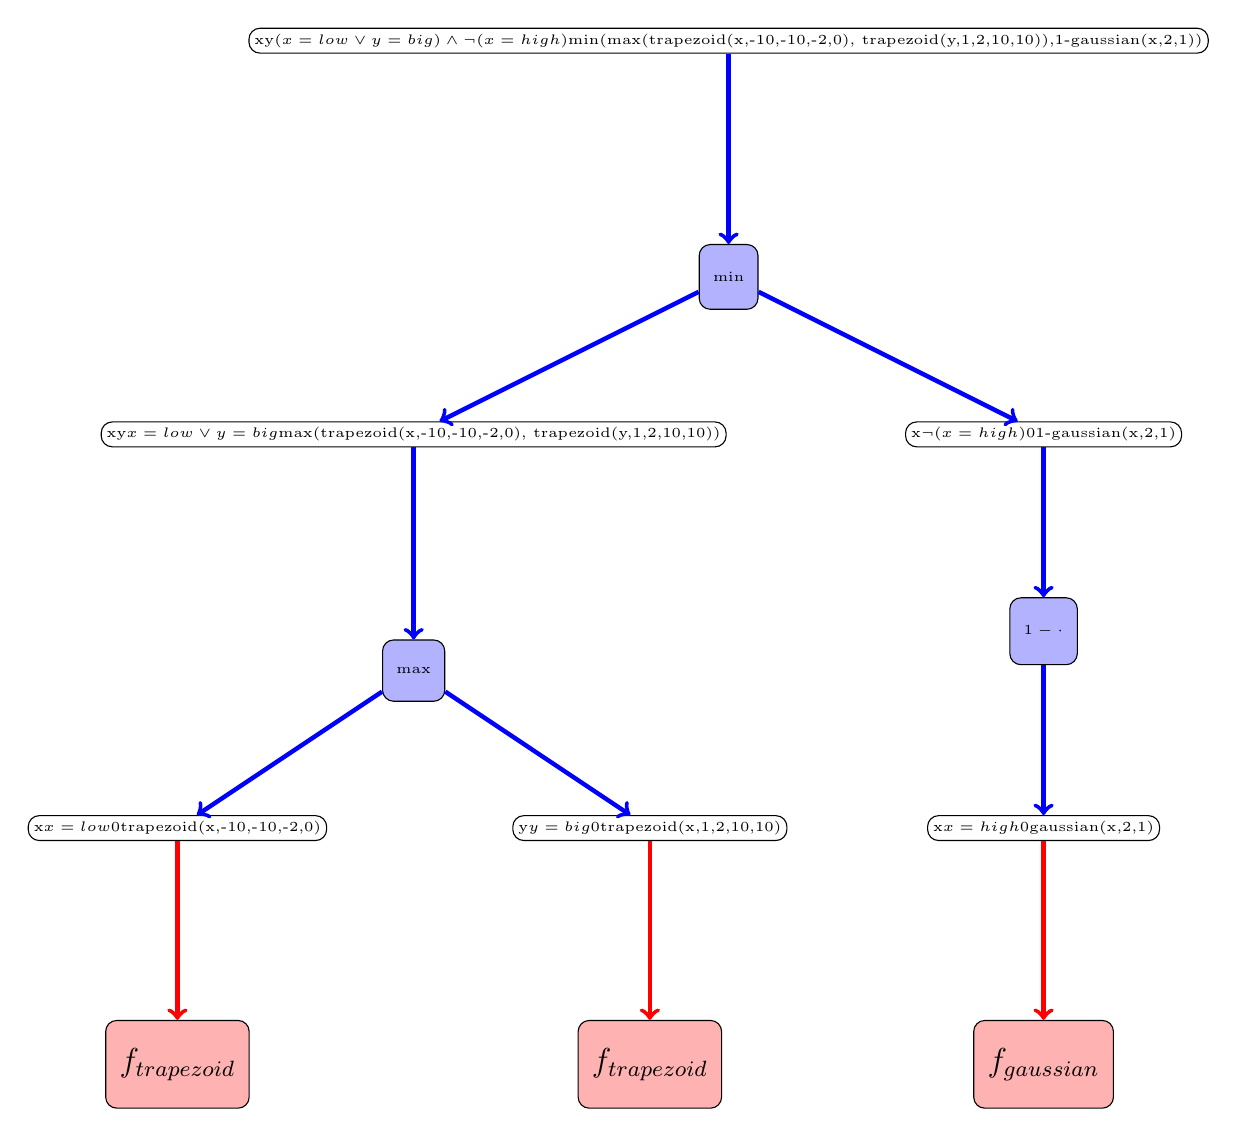
\begin{tikzpicture}[scale=2,font=\tiny]


    \node [rectangle, rounded corners, draw, inner sep=2pt] (A) at (0,0) {
      \fuzzySetNodeTwoD{x}{y}{$(x=low \lor y=big) \land \neg (x = high)$}{min(max(trapezoid(x,-10,-10,-2,0), trapezoid(y,1,2,10,10)),1-gaussian(x,2,1))}
    };

    \node [rectangle,rounded corners,draw,inner sep=5pt, inner ysep=10pt,fill=blue!30] (X) at (0,-1.5) {
      $\min$
    };


    \node [rectangle,rounded corners,draw,inner sep=2pt] (B) at (-2,-2.5) {
      \fuzzySetNodeTwoD{x}{y}{$x=low \lor y=big$}{max(trapezoid(x,-10,-10,-2,0), trapezoid(y,1,2,10,10))}
    };

    \node [rectangle,rounded corners,draw,inner sep=2pt] (C) at (2,-2.5) {
      \fuzzySetNodeOneD{x}{$\neg (x = high)$}{0}{1-gaussian(x,2,1)}
    };


    \node [rectangle,rounded corners,draw,inner sep=5pt, inner ysep=10pt,fill=blue!30] (Y) at (-2,-4) {
      $\max$
    };

    \node [rectangle,rounded corners,draw,inner sep=5pt, inner ysep=10pt,fill=blue!30] (Z) at (2,-3.75) {
      $1 - \cdot$
    };


    \node [rectangle,rounded corners,draw,inner sep=2pt] (D) at (-3.5,-5) {
      \fuzzySetNodeOneD{x}{$x = low$}{0}{trapezoid(x,-10,-10,-2,0)}
    };

    \node [rectangle,rounded corners,draw,inner sep=2pt] (E) at (-0.5,-5) {
      \fuzzySetNodeOneD{y}{$y = big$}{0}{trapezoid(x,1,2,10,10)}
    };

    \node [rectangle,rounded corners,draw,inner sep=2pt] (F) at (2,-5) {
      \fuzzySetNodeOneD{x}{$x = high$}{0}{gaussian(x,2,1)}
    };



    \node [rectangle,rounded corners,draw,inner sep=5pt, inner ysep=10pt,fill=red!30] (G) at (-3.5,-6.5) {
      \large $f_{trapezoid}$
    };

    \node [rectangle,rounded corners,draw,inner sep=5pt, inner ysep=10pt,fill=red!30] (H) at (-0.5,-6.5) {
      \large $f_{trapezoid}$
    };

    \node [rectangle,rounded corners,draw,inner sep=5pt, inner ysep=10pt,fill=red!30] (I) at (2,-6.5) {
      \large $f_{gaussian}$
    };


    \draw[->,ultra thick,draw = blue] (A) -- (X);
    \draw[->,ultra thick,draw = blue] (X) -- (B);
    \draw[->,ultra thick,draw = blue] (X) -- (C);


    \draw[->,ultra thick,draw = blue] (B) -- (Y);
    \draw[->,ultra thick,draw = blue] (Y) -- (D);
    \draw[->,ultra thick,draw = blue] (Y) -- (E);

    \draw[->,ultra thick,draw = blue] (C) -- (Z);
    \draw[->,ultra thick,draw = blue] (Z) -- (F);

    \draw[->,ultra thick,draw = red] (D) -- (G);
    \draw[->,ultra thick,draw = red] (E) -- (H);
    \draw[->,ultra thick,draw = red] (F) -- (I);
  \end{tikzpicture}

  \caption[Example of modular fuzzy set construction]{Recursive construction of a complex fuzzy set from simpler fuzzy sets. Using the linguistic variables $x$ with the terms $\{low, high\}$ and $y$ with the terms $\{big, small\}$ we can construct the fuzzy set $(x=low \lor y=big) \land \neg (x = high)$ by combining the fuzzy sets $x=low \lor y=big$ and $\neg (x = high)$. Those fuzzy sets are again constructed from the simpler fuzzy sets $x=low$, $y=big$ and $x=high$.

    The fuzzy sets at the leaf level can be directly constructed using predefined \textcolor{red}{\texttt{BaseMembershipFunctions}} (e.g., trapezoid, sigmoid, gaussian \dots) and provide the foundation for the more complex fuzzy sets
    All other fuzzy sets are created by combining other fuzzy sets using \textcolor{blue}{\texttt{CompositeMembershipFunctions}}. The logical operators $\min$, $\max$, and $1 - \cdot$ are implemented this way, as they directly act on top of other fuzzy sets.}
  \label{fig:modularfuzzysetconstruction}
\end{figure}

\begin{figure}[H]
  \centering
  \includesvg[width=\textwidth]{figures/class-diagram.svg}
  \caption[Class diagram of the Fuzzy Tuning Strategy]{Simplified class diagram of the Fuzzy Tuning strategy. There is a clear separation between implementing the Fuzzy Logic framework and the tuning strategy. This allows for an easy reuse of the Fuzzy Logic framework in other parts of AutoPas if desired.}
  \label{fig:classdiagram}
\end{figure}


\section{Rule Parser}

The Rule Parser is responsible for parsing the rule base supplied by the user and converting it into the internal representation used by the Fuzzy Tuning framework. It uses the ANTLR4\footnote{https://www.antlr.org/} parser generator to create a parser for a domain-specific language tailored to the needs of the Fuzzy Tuning. The language is inspired by common standards such as the Fuzzy Control Language (FCL)\footnote{https://www.fuzzylite.com/} but is designed to be more lightweight and directly incorporate aspects of the AutoPas simulation.
The parsed rules are transformed into the internal representation by a visitor pattern that traverses the parse tree generated by ANTLR4 and internally builds the corresponding object hierarchy.

\section{Tuning Strategy}

The Tuning Strategy implements the interface between the Fuzzy Tuning framework and the AutoPas simulation and is responsible for updating the configuration queue of configurations to be tested next.

It does this by evaluating all fuzzy systems present in the rule file with the current information on the simulation. It primarily used \emph{LiveInformation} data, containing summary statistics about various aspects of the current simulation state. Possible parameters include the total number of particles, the average density, or the average homogeneity of the particle distribution. Each evaluation of a Fuzzy Control System yields a single numeric value, which is then passed on to the \texttt{OutputMapper}, which determines the resulting configuration. Such a mapping is necessary because the output of the Fuzzy Control System is a continuous value, while the configuration space of AutoPas is discrete, and we need to define mappings between the two.

This method of assigning concrete configurations to the continuous output space of the Fuzzy Control Systems is inspired by Mohammed et al.~\cite{Mohammed2022}'s work on scheduling algorithms. Internally, the \texttt{OutputMapper} stores an ideal location for each available configuration and determines the configuration closest to the predicted value.

The resulting list of configurations predicted by the Fuzzy Tuning Strategy is then used to update AutoPas's configuration queue. In the following iterations, all of those configurations are used to run a few steps of the simulation, and the configuration with the best performance is then used for the following simulation phase.

Currently, two different modes of interpreting the rules are implemented:

\subsection{Component Tuning Approach}

The component Tuning Approach expects a single Fuzzy Control System for each tunable parameter. All those Fuzz Systems should then attempt to predict the best value of their parameter independent of the other parameters. This approach requires the rule file to only define $\#Parameters$ different Fuzzy Control Systems, which makes it easier to maintain and understand. An obvious drawback of this method is the independence assumption between the parameters, which might not hold in practice.

Another problem of this approach lies in the defuzzification step. As this method relies on defining a single system for all parameter values, there must be a \emph{ranking} of all those values on a single numeric scale. Such a ranking is problematic, as most tunable values are nominal and do not have a natural order. To circumvent this problem, we can use a defuzzification method that does not perform interpolations between the values. Using such a method, the placement of the linguistic terms can be arbitrary. One such method is \gls{mom}. It selects the mean of all $x$-values for which the membership function is maximal. When using Gaussian-shaped membership functions, this method will only ever return the mean of the Gaussian with the highest activation. The OutputMapper can directly take these values and assign them to the corresponding nominal value of the tunable parameter. All predicted values are then used to filter the configuration queue, excluding all configurations that do not match the predicted values.

\autoref{fig:fuzzyInferenceSystemIndividual} shows a schematic of the Component Tuning Approach.


\begin{figure}[H]
  \centering

  \newcommand{\xShift}{0.15}
  \newcommand{\yShift}{0.27}
  \newcommand{\scaleShift}{0.1}
  \begin{tikzpicture}[scale=2,font=\small]
    \node[anchor=east] (L) at (-3,-0.6) {$\text{LiveInfo} \in \mathbb{R}^d$};

    \foreach \name [count=\i from 0] in { Newton3, DataLayout, Traversal, Container}
      {
        \pgfmathsetmacro{\scaleFactor}{1 + \i*\scaleShift}

        \node [rectangle,rounded corners,draw,inner sep=2pt,fill=white!80!black,scale=\scaleFactor,anchor=east] (A) at (0-\i * \xShift,0-\i * \yShift) {
          \begin{tikzpicture}[font=\small]
            \begin{axis}%
              [
                title={FCS [\name]},
                width=3.8cm,
                height=2.2cm,
                axis lines=center,
                xmin=0,
                xmax=4,
                xlabel={$\mathbb{R}$},
                x label style={at={(axis description cs:1,0.2)},anchor=west},
                ylabel=$\mu$,
                y label style={at={(axis description cs:0,0.8)},anchor=east},
                xtick={},
                xticklabels= {},
                ytick={},
                yticklabels={},
                ymax=1,
                every axis plot/.append style={thick},
                domain=0:4
              ]
              \addplot[blue, samples=17] {gaussian(x,1,0.2)};
              \addplot[red,samples=15] {gaussian(x,2,0.2)};
              \addplot[green,samples=17] {gaussian(x,3,0.2)};
            \end{axis}
          \end{tikzpicture}
        };

        \node [rectangle,rounded corners,draw,inner sep=2pt,fill=white!80!black,scale=\scaleFactor*1.1,anchor=east] (O) at (1.45-\i *\xShift*0.2,0-\i*\yShift) {\tiny{OutputMapper}};

        \node[scale=\scaleFactor*1.2, anchor=west] (T) at (1.85-\i*\xShift*0.3,0-\i*\yShift) {\tiny{\name Option}};

        \draw[->, thick] (L.east) -- (A.west) ;

        \draw[->, thick] (A.east) -- (O.west) ;
        \draw[->, thick] (O.east) -- (T.west) ;
      }

  \end{tikzpicture}

  \caption[Visualization of the fuzzy control systems for the Component Tuning Approach]{Example Visualization of the fuzzy control systems for the Component Tuning Approach. The parameters \texttt{Container}, \texttt{Traversal}, \texttt{DataLayout}, and \texttt{Newton3} are tuned independently. The OutputMapper assigns the predicted values to the corresponding nominal values of the parameters.}
  \label{fig:fuzzyInferenceSystemIndividual}

\end{figure}


\subsection{Suitability Tuning Approach}

The Suitability Approach differs from the Component Tuning Approach in that it utilizes $\#Container\_options \cdot \#Traversal\_options \cdot \#DataLayout\_options \cdot \#Newton3\_options$ different Fuzzy Control Systems, one for each possible combination of those parameters. Consequently, there are way more Fuzzy Control Systems to evaluate. The advantage of this approach is that there is no need to rank the output values, and one can utilize the power of interpolation between different predictions by using the \gls{cog} defuzzification method as the predicted suitabilities have a natural order. Furthermore, dependencies and incompatibilities between the parameters can be modeled accurately. The downside is the increased complexity of the rule file, which quickly becomes infeasible to maintain by hand. Surprisingly, the cost of evaluating all those Fuzzy Control Systems is negligible compared to the overhead of other tuning strategies.

Each System is responsible for predicting the suitability of a specific configuration, ranging from 0 (not suitable) to 100\% (perfectly suitable). After applying the OutputMapping, the Strategy selects all configurations performing within a certain threshold of the best configuration and rewrites the configuration queue accordingly. \autoref{fig:fuzzyInferenceSystemSuitability} shows a schematic of the Suitability Tuning Approach.

\begin{figure}[H]
  \centering

  \newcommand{\xShift}{0.03}
  \newcommand{\yShift}{0.13}
  \newcommand{\scaleShift}{0.066}

  \begin{tikzpicture}[scale=2,font=\small]
    \node[anchor=east] (L) at (-3.5,-1.5) {$\text{LiveInfo} \in \mathbb{R}^d$};

    \foreach \name [count=\i from 0] in {15,...,1}
      {
        \pgfmathsetmacro{\scaleFactor}{1 + \i*\scaleShift}
        \pgfmathsetmacro{\opacity}{0 + 1*\i/6}
        \pgfmathsetmacro{\arrowThickness}{0.2 + 1.8*\i/16}


        \node [rectangle,rounded corners,draw,inner sep=2pt,fill=white!80!black, fill opacity=\opacity, draw opacity=\opacity,scale=\scaleFactor,anchor=east] (A) at (0-\i * \xShift,0-\i * \yShift) {
          \begin{tikzpicture}[font=\tiny]
            \begin{axis}%
              [
                title={FCS [Combination\textsubscript {\ifthenelse{\name<10}{\name\space}{\name}}]},
                width=3cm,
                height=2cm,
                axis lines=center,
                xmin=0,
                xmax=4,
                xlabel={$\mathbb{R}$},
                x label style={at={(axis description cs:1,0.2)},anchor=west},
                ylabel=$\mu$,
                y label style={at={(axis description cs:0,0.8)},anchor=east},
                xtick={},
                xticklabels= {},
                ytick={},
                yticklabels={},
                ymax=1,
                every axis plot/.append style={thick},
                domain=0:4
              ]
              \addplot[blue, samples=17] {gaussian(x,1,0.2)};
              \addplot[red,samples=15] {gaussian(x,2,0.2)};
              \addplot[green,samples=17] {gaussian(x,3,0.2)};
            \end{axis}
          \end{tikzpicture}
        };

        \node [rectangle,rounded corners,draw,inner sep=2pt,fill=white!80!black, fill opacity=\opacity, draw opacity=\opacity,scale=\scaleFactor*0.8,anchor=east] (O) at (1+\i *\xShift*1,0-\i*\yShift) {\tiny{OutputMapper}};

        \node[scale=\scaleFactor*0.8,fill opacity=\opacity, draw opacity=\opacity, anchor=west] (T) at (1.3+\i*\xShift*1,0-\i*\yShift) {\tiny{ Configuration {\ifthenelse{\name<10}{\name\space}{\name}}}};

        \node[scale=\scaleFactor*0.8,fill opacity=\opacity, draw opacity=\opacity, anchor=west] (S) at (1.25+\i*\xShift*1,-0.2-\i*\yShift) {};

        \draw[->,thick,fill opacity=\opacity, draw opacity=\opacity,] (L.east) -- (A.west) ;

        \draw[->,thick,fill opacity=\opacity, draw opacity=\opacity,] (A.east) -- (O.west) ;
        \draw[->,thick,fill opacity=\opacity, draw opacity=\opacity,] (O.east) -- (T.west) ;

        \draw[thick, fill opacity=\opacity, draw opacity=\opacity]
        (A.east) edge[bend right, looseness=0.5, ->]
        (S.south west) ;
      }

  \end{tikzpicture}

  \caption[Visualization of the fuzzy control systems for the Suitability Tuning Approach]{Example Visualization of the fuzzy control systems for the Suitability Tuning Approach. Each Fuzzy Control System is responsible for predicting the suitability of a specific configuration. The suitability and the mapped configuration are passed on to the Strategy, which only considers highly suitable configurations for the next simulation steps.}
  \label{fig:fuzzyInferenceSystemSuitability}
\end{figure}


\chapter{Proof of Concept}
\label{sec:proof_of_concept}

% -------------------------------------------------------------------------------

% parameers: xlabel, center
\newcommand{\fuzzyTreeNode}[2]{
    \begin{tikzpicture}
        \begin{axis}%
            [
                title = {Fuzzy Split: $#1 \leq #2$},
                width=4.5cm,
                height=3cm,
                axis lines=center,
                xlabel={#1},
                x label style={at={(axis description cs:0.9,-0.1)},anchor=north},
                ylabel=$\mu$,
                y label style={at={(axis description cs:0.5,1)},anchor=south},
                xmin=-5,
                xmax=5,
                xtick={},
                xticklabels= {},
                ytick={},
                yticklabels={},
                extra x ticks={0},
                extra x tick labels={#2},
                ymax=1,
                samples=50,
                extra y ticks={1},
                every axis plot/.append style={thick}
            ]
            \addplot[red]  {sigmoid(x,0,-1)};
            \addplot[blue] {sigmoid(x,0,1)};
            \node[anchor=center, red] at (axis cs:-2.9,0.6) {$\mu_{\text{#1smaller#2}}$};
            \node[anchor=center, blue] at (axis cs:3.1,0.6) {$\mu_{\text{#1greater#2}}$};
        \end{axis}

    \end{tikzpicture}
}

\newcommand{\fuzzyTreeLeaf}[1]{
    \begin{tikzpicture}
        \begin{axis}%
            [
                title = {Class: #1},
                width=3.25cm,
                height=2.25cm,
                axis lines=center,
                xlabel={$\text{class}$},
                x label style={at={(axis description cs:0.6,-0.3)},anchor=west},
                ylabel=$\mu$,
                y label style={at={(axis description cs:0.5,1)},anchor=south},
                xmin=-5,
                xmax=5,
                xtick={},
                xticklabels= {},
                ytick={},
                yticklabels={},
                extra x ticks={0},
                extra x tick labels={#1},
                ymax=1,
                samples=10,
                extra y ticks={1},
                every axis plot/.append style={thick}
            ]
            \addplot[black]  {gaussian(x,0,1)};
        \end{axis}

    \end{tikzpicture}
}

% parameers: xlabel, center
\newcommand{\crispTreeNode}[2]{
    \begin{tikzpicture}
        \begin{axis}%
            [
                title = {Crisp Split: $#1 \leq #2$},
                width=4.5cm,
                height=3cm,
                axis lines=center,
                xlabel={#1},
                x label style={at={(axis description cs:0.9,-0.1)},anchor=north},
                ylabel=$\mu$,
                y label style={at={(axis description cs:0.5,1)},anchor=south},
                xmin=-5,
                xmax=5,
                xtick={},
                xticklabels= {},
                ytick={},
                yticklabels={},
                extra x ticks={0},
                extra x tick labels={#2},
                ymin=-0.1,
                ymax=1.1,
                samples=50,
                extra y ticks={1},
                every axis plot/.append style={thick}
            ]
            \addplot[red,domain=-5:-0.6] {step(x,0,-1)};
            \addplot[blue,domain=0.6:5] {step(x,0,1)};
            \addplot[red,domain=0.6:5] {step(x,0,-1)};
            \addplot[blue,domain=-5:-0.6] {step(x,0,1)};

            \node[draw,draw=black,circle,inner sep=1pt,minimum width=3pt,thick] at (axis cs:0,1) {};
            \node[draw,draw=black,circle,inner sep=1pt,minimum width=3pt,thick] at (axis cs:0,0) {};

            \node[anchor=center, red] at (axis cs:-2.9,0.6) {$#1 \leq #2$};
            \node[anchor=center, blue] at (axis cs:3.1,0.6) {$#1 > #2$};
        \end{axis}

    \end{tikzpicture}
}


% -------------------------------------------------------------------------------

This chapter presents a proof of concept for the fuzzy tuning technique. We will develop two different knowledge bases to predict the optimal configurations for \texttt{\gls{mdflexible}} simulations.

As for all fuzzy systems, creating the knowledge base is one of the most complex parts of developing a fuzzy system, as it typically requires a profound understanding of the system to create meaningful rules. Luckily, methods such as data-driven approaches exist to semi-automate this process. This is extremely useful as those methods do not require prior expert knowledge about the system. For a problem as complex as tuning molecular dynamics simulations, it would be extremely hard to create a meaningful knowledge base from scratch. Such data-driven methods provide a good initial set of rules that experts can manually evaluate and adjust if desired. In this work, we will use a decision tree approach proposed by Crockett et al.~\cite{CROCKETT20062809}. This proposed method uses machine learning to first train decision trees on the dataset to create an initial crisp rule base. In the second step, the decision trees are converted into so-called fuzzy decision trees, which can then be used to extract the linguistic variables and fuzzy rules.


\subsection{Decision Trees}

Decision trees are prevalent machine learning algorithms used for classification and regression tasks. They work by recursively partitioning the input using axis-parallel splits so that the resulting subsets are as pure as possible. Concretely, they try to minimize a given impurity metric, such as the Gini impurity $I_G = \sum_{i=1}^{n} p_i(1-p_i)$ or the entropy $H = -\sum_{i=1}^{n} p_i \log_2(p_i)$ of the subsets~\cite{10.5555/2380985}. The probability $p_i$ is the fraction of samples in the subset that belong to class $i$, and $n$ is the total number of classes.

Since decision trees directly partition the input space into regions with different classes, they can also be depicted using their decision surface if the dimensionality allows it. The decision surface of a decision tree is a piecewise constant function that assigns the predicted class label to each point in the input space of the decision tree. An example decision tree and its decision surface are shown in \autoref{fig:decisionTreeExample} and \autoref{fig:decisionBoundaryExample}.

% Image of a decision tree
\begin{multicols}{2}
    \begin{figure}[H] % [H] for HERE
        \centering
        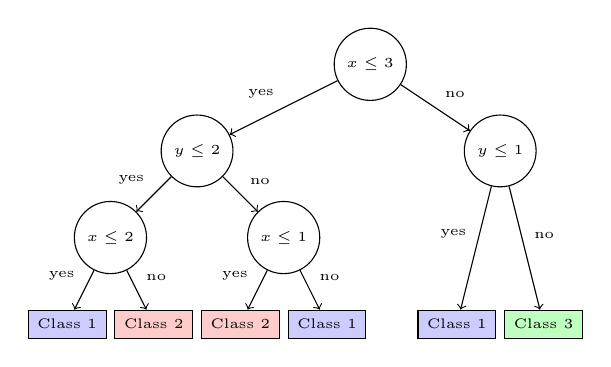
\begin{tikzpicture}[scale=1.1,font=\tiny]
            \node [circle, draw] (A) at (0,0) {$x \leq 3$};
            \node [circle, draw] (B) at (-2,-1) {$y \leq 2$};
            \node [circle, draw] (C) at (1.5,-1) {$y \leq 1$};
            \node [circle, draw] (D) at (-3,-2) {$x \leq 2$};
            \node [circle, draw] (E) at (-1,-2) {$x \leq 1$};

            \node [rectangle,draw,fill=blue!20] (F) at (-3.5,-3) {Class 1};
            \node [rectangle,draw,fill=red!20] (G) at (-2.5,-3) {Class 2};
            \node [rectangle,draw,fill=red!20] (H) at (-1.5,-3) {Class 2};
            \node [rectangle,draw,fill=blue!20] (I) at (-0.5,-3) {Class 1};
            \node [rectangle,draw,fill=blue!20] (J) at (1,-3) {Class 1};
            \node [rectangle,draw,fill=green!25] (K) at (2,-3) {Class 3};

            \draw[->] (A) -- (B) node [midway, left, above left] {yes};
            \draw[->] (A) -- (C) node [midway, right, above right] {no};
            \draw[->] (B) -- (D) node [midway, left, above left] {yes};
            \draw[->] (B) -- (E) node [midway, right, above right] {no};

            \draw[->] (C) -- (J) node [midway, left, above left] {yes};
            \draw[->] (C) -- (K) node [midway, right, above right] {no};

            \draw[->] (D) -- (F) node [midway, left, above left] {yes};
            \draw[->] (D) -- (G) node [midway, right, above right] {no};

            \draw[->] (E) -- (H) node [midway, left, above left] {yes};
            \draw[->] (E) -- (I) node [midway, right, above right] {no};

        \end{tikzpicture}

        \caption[Decision tree used for the example]{An example decision tree for a dataset with two features $x$ and $y$. There are three distinct classes in the dataset}
        \label{fig:decisionTreeExample}
    \end{figure}

    \columnbreak    % start next column

    \begin{figure}[H]
        \centering
        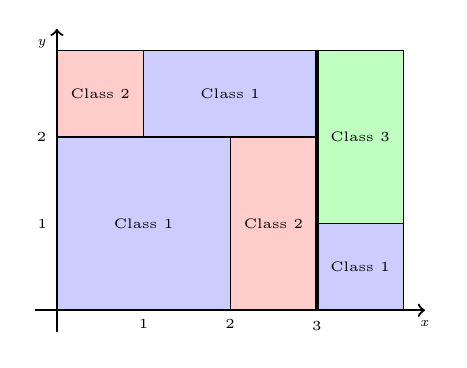
\begin{tikzpicture}[scale=1.1,font=\tiny]

            \draw[fill=red!20] (0,2) -- (1,2) -- (1,3) -- (0,3) -- cycle;

            \draw[fill=blue!20] (1,2) -- (3,2) -- (3,3) -- (1,3) -- cycle;

            \draw[fill=blue!20] (0,0) -- (2,0) -- (2,2) -- (0,2) -- cycle;
            \draw[fill=red!20] (2,0) -- (3,0) -- (3,2) -- (2,2) -- cycle;

            \draw[fill=blue!20] (3,0) -- (4,0) -- (4,1) -- (3,1) -- cycle;
            \draw[fill=green!25] (3,1) -- (4,1) -- (4,3) -- (3,3) -- cycle;

            \draw[->, thick] (-0.25,0) -- (4.25,0) node [below] {\textit{x}};
            \draw[->, thick] (0,-0.25) -- (0,3.25) node [below left] {\textit{y}};

            % decision lines

            \draw[line width=1.5pt,] (3,0) node [below] {3}  -- (3,3) ;
            \draw[line width=1pt] (0,2) node [left] {2} -- (3,2);

            \draw[] (2,0) node [below] {2}-- (2,2);

            \node [below] at (1,0) {1};

            \node [left] at (0,1) {1};

            % area labels
            \node [] at (0.5,2.5) {Class 2};
            \node [] at (2,2.5) {Class 1};

            \node [] at (1,1) {Class 1};
            \node [] at (2.5,1) {Class 2};


            \node [] at (3.5,2) {Class 3};
            \node [] at (3.5,0.5) {Class 1};

        \end{tikzpicture}
        \caption[Decision surface of the example decision tree]{The decision surface of the decision tree from \autoref{fig:decisionTreeExample} on $\mathcal{D}=[0,4]\times[0,3]$. }
        \label{fig:decisionBoundaryExample}
    \end{figure}
\end{multicols}


\subsection{Conversion of Decision Trees to Fuzzy Control Systems}

This section will demonstrate how to convert a classical decision tree into a fuzzy decision system using the fictional decision tree from \autoref{fig:decisionTreeExample} as an example.

\subsubsection{Fuzzy Decision Trees}

As the conversion makes use of so-called fuzzy decision trees, we will briefly introduce them here. Fuzzy decision trees are a generalization of classical decision trees and allow for fuzzy logic to be used in the decision-making process. Instead of following the classical \texttt{if then else} logic to descend into the decision tree, it uses fuzzy sets at each node of the tree to fuzzily calculate the contribution of each branch to the final decision based on the degree of truth of both possible paths. Contrary to classical decision trees, which follow a single path from the root to a leaf node, fuzzy decision trees explore all possible paths simultaneously and make a final decision by aggregating the results of the paths using fuzzy logic operations.

\subsubsection{Conversion}


A classical decision tree is converted into a fuzzy decision tree by replacing the crisp decision (e.g., $x \leq 3$) at each internal node of the decision tree with a fuzzy set. Those fuzzy sets should maintain the same semantics as the crisp decision but should provide a continuous value in the range $[0,1]$ specifying the degree of how much each branch should be considered. Classical decision trees can only make binary decisions (${0,1}$), which causes them to only consider a single path of the decision tree. Allowing them to consider multiple paths simultaneously can drastically increase the decision-making capabilities of the decision tree, especially in boundary cases where the decision can be ambiguous.


The shape of the membership functions of the fuzzy sets can be chosen arbitrarily, but since trees work with one-sided boundaries, typical choices include complementary \texttt{sigmoid}-shaped functions that are centered around the crisp decision boundary (See \autoref{fig:fuzzyMembershipFunctions}), as those function shapes maintain the semantics of the branching idea. Crockett et al.~\cite{CROCKETT20062809} suggested creating those sigmoid shapes with a \emph{width} proportional to the standard deviation of the attribute. In Particular, the authors suggested an interval $[t-n\cdot \sigma, t+n\cdot \sigma]$ for the membership function, where  $t$ is the value of the decision boundary, $\sigma$ is the standard deviation of the attribute and $n$ is a parameter that can be adjusted to control the \emph{width} of the membership function. This interval specifies the region of the membership function where most of the change in membership occurs. The value of $n$ is typically chosen from the interval $n\in [0,5]$ as the membership function can become too broad otherwise and could even weaken the decision-making process~\cite{CROCKETT20062809}. In this work, we will use $n=2$ as a default value. Using this method, it is possible to fully automate the conversion of a decision tree into a fuzzy decision tree, which we will utilize in this work.


\begin{figure}[h]
    \centering
    \begin{tikzpicture}[scale=2,font=\tiny]
        \node [rectangle,rounded corners,draw,inner sep=2pt] (A) at (0.5,0) {
            \crispTreeNode{x}{3}
        };

        \node [rectangle,rounded corners,draw,inner sep=2pt] (B) at (3.5,0) {
            \fuzzyTreeNode{x}{3}
        };

        \path[draw=black, line width=1mm, -{Triangle[length=4mm, bend]}]
        (1.5,0) to [bend left] (2.5,0);

        \path[draw=white, line width=0.5mm, -{Triangle[length=3.25mm, bend, angle'=60]}, shorten >= 0.5mm, shorten <= 0.25mm]
        (1.5,0) to [bend left] (2.5,0);

    \end{tikzpicture}
    \caption[Conversion of crisp tree node into fuzzy tree node]{Conversion of crisp set membership functions to fuzzy set membership functions. The classical membership functions $x \leq 3$ and $x>3$ of a decision tree node are replaced by two \texttt{sigmoid}-shaped membership functions \textcolor{red}{$\mu_{\text{xsmaller3}}$} and \textcolor{blue}{$\mu_{\text{xgreater3}}$} that specify to which degree one should traverse left or right. The \emph{width} of the membership functions is data dependent and is determined by $n\cdot \sigma = 2 \cdot \sigma$. }
    \label{fig:fuzzyMembershipFunctions}
\end{figure}

Once the internal nodes of the decision tree have been converted, the next step is to convert the leaf nodes of the decision tree to fuzzy leaf nodes. As the outputs of decision trees are specific class labels, we can define a single linguistic variable consisting of all possible class labels together with a corresponding fuzzy set. The shapes of the membership functions for the fuzzy sets can again be chosen mostly arbitrarily, but we will use \texttt{gaussian} functions with a different mean as they are a good choice for representing class labels in a continuous domain. This way of placing the fuzzy sets is not directly obvious, and the placement can significantly influence the defuzzification process depending on the chosen defuzzification function, as we will see later. However, we can minimize this issue by carefully choosing a suitable defuzzification method.
The resulting conversion of the decision tree in \autoref{fig:decisionTreeExample} into a fuzzy decision tree is shown in \autoref{fig:fuzzyDecisionTreeExample}.


\begin{figure}[h!]
    \centering
    \begin{tikzpicture}[scale=1.9,font=\tiny]

        \node [rectangle, rounded corners, draw, inner sep=2pt] (A) at (0,0) {
            \fuzzyTreeNode{x}{3}
        };

        \node [rectangle,rounded corners,draw,inner sep=2pt] (B) at (-2,-1.6) {
            \fuzzyTreeNode{y}{2}
        };

        \node [rectangle,rounded corners,draw,inner sep=2pt] (C) at (1.8,-1.6) {
            \fuzzyTreeNode{y}{1}
        };

        \node [rectangle,rounded corners,draw,inner sep=2pt] (D) at (-3,-3.2) {
            \fuzzyTreeNode{x}{2}
        };

        \node [rectangle,rounded corners,draw,inner sep=2pt] (E) at (-1,-3.2) {
            \fuzzyTreeNode{x}{1}
        };


        \node [rectangle,rounded corners,draw,inner sep=2pt,fill=blue!20] (F) at (-3.7,-4.7) {
            \fuzzyTreeLeaf{1}
        };

        \node [rectangle,rounded corners,draw,inner sep=2pt,fill=orange!20] (G) at (-2.6,-4.7) {
            \fuzzyTreeLeaf{2}
        };

        \node [rectangle,rounded corners,draw,inner sep=2pt,fill=orange!20] (H) at (-1.5,-4.7) {
            \fuzzyTreeLeaf{2}
        };

        \node [rectangle,rounded corners,draw,inner sep=2pt,fill=blue!20] (I) at (-0.4,-4.7) {
            \fuzzyTreeLeaf{1}
        };

        \node [rectangle,rounded corners,draw,inner sep=2pt,fill=blue!20] (J) at (1.25,-4.7) {
            \fuzzyTreeLeaf{1}
        };

        \node [rectangle,rounded corners,draw,inner sep=2pt,fill=green!20] (K) at (2.35,-4.7) {
            \fuzzyTreeLeaf{3}
        };



        \draw[->] (A) -- (B) node [pos=.4, left, above left] {yes};
        \draw[->] (A) -- (C) node [pos=.4, right, above right] {no};

        \draw[->] (B) -- (D) node [pos=.8, left, above left] {yes};
        \draw[->] (B) -- (E) node [pos=.8, right, above right] {no};

        \draw[->] (C) -- (J) node [pos=.2, left, above left] {yes};
        \draw[->] (C) -- (K) node [pos=.2, right, above right] {no};

        \draw[->] (D) -- (F) node [pos=.6, left, above left] {yes};
        \draw[->] (D) -- (G) node [pos=.6, right, above right] {no};

        \draw[->] (E) -- (H) node [pos=.6, left, above left] {yes};
        \draw[->] (E) -- (I) node [pos=.6, right, above right] {no};
    \end{tikzpicture}

    \caption[Fuzzy decision tree created from the regular decision tree]{The fuzzy decision tree corresponding to the decision tree in \autoref{fig:decisionTreeExample}. Internal nodes use two \texttt{sigmoid} membership functions (\textcolor{red}{$\mu_{\text{smaller}}$} and \textcolor{blue}{$\mu_{\text{greater}}$}) instead of a crisp decision. The leaf nodes use different \texttt{gaussian} membership functions centered around a unique mean.}

    \label{fig:fuzzyDecisionTreeExample}
\end{figure}

It is now possible to fully extract all linguistic variables from the fuzzy decision tree. Every fuzzy set defined over the same variable can be collected into a single linguistic variable. This results in linguistic variables consisting of a bunch of different \texttt{sigmoid} membership functions for input variables (internal nodes) and a single linguistic variable with different \texttt{gaussian} membership functions for the output variable (leaf nodes). The resulting linguistic variables are shown in \autoref{fig:fuzzyDecisionTreeLinguisticVariables}.


\begin{figure}[h]
    \centering

    \includegraphics[width=\linewidth]{figures/ProofOfConcepts/fuzzy_sets.png}

    \caption[Linguistic variables for the converted fuzzy decision tree]{Linguistic variables used in the fuzzy decision tree of \autoref{fig:fuzzyDecisionTreeExample}. The standard deviation of the attributes is assumed to be $\sigma \approx 0.5$ such that the \emph{width} of the sigmoid membership functions is $n\cdot \sigma \approx 1$. The standard deviation of the class values is chosen so that they do not overlap too much.}
    \label{fig:fuzzyDecisionTreeLinguisticVariables}
\end{figure}

\subsubsection{Rule Extraction}

The final step is to extract the fuzzy rules from the tree. This can be done by traversing the tree in a depth-first manner and collecting the correct membership functions for each path ending in a leaf node along the way. As all conditions of this path have to hold simultaneously, all fuzzy sets are connected using the \texttt{AND} operation. This newly created fuzzy set, which consists of the intersection of all fuzzy sets along the way, is the premise of selecting the fuzzy set of the leaf node. Consequently, both fuzzy sets are connected using the Mamdani \texttt{IMPLICATION} operator. This implication then forms a rule for the fuzzy system. Therefore, each unique path traversing the tree results in a unique rule. This process essentially mimics the decision surface seen in \autoref{fig:decisionBoundaryExample}, as we create precisely one rule for each region of the decision surface. The rules extracted from the fuzzy decision tree in \autoref{fig:fuzzyDecisionTreeExample} using this method are shown in \autoref{tab:fuzzyRulesExample}.


\newpage
\newcommand{\is}{\textit{ is }}


\begin{table}[H]
    \centering
    \begin{tabular}{c|l|c}
        \textbf{Rule} & \textbf{Antecedent}                                                             & \textbf{Consequent} \\
        \hline
        1             & $x \is \text{smaller3} \land y \is \text{smaller2} \land x \is \text{smaller2}$ & $class \is 1$       \\
        2             & $x \is \text{smaller3} \land y \is \text{smaller2} \land x \is \text{greater2}$ & $class \is 2$       \\
        3             & $x \is \text{smaller3} \land y \is \text{greater2} \land x \is \text{smaller1}$ & $class \is 2$       \\
        4             & $x \is \text{smaller3} \land y \is \text{greater2} \land x \is \text{greater1}$ & $class \is 1$       \\
        5             & $x \is \text{greater3} \land y \is \text{smaller1}$                             & $class \is 1$       \\
        6             & $x \is \text{greater3} \land y \is \text{greater1}$                             & $class \is 3$       \\
    \end{tabular}
    \caption[Extracted fuzzy rules from the fuzzy decision tree]{Extracted fuzzy rules from the fuzzy decision tree in \autoref{fig:fuzzyDecisionTreeExample} in the format: $\textbf{IF} \text{ Antecedent } \textbf{THEN} \text{ Consequent }$}
    \label{tab:fuzzyRulesExample}
\end{table}

\subsubsection{Fuzzy Control System}

With the linguistic variables and fuzzy rules extracted from the decision tree, we can finally use them to create a fuzzy system that can predict the class of a new data point based on its features. Since the fuzzy system can be seen as a black box mapping continuous input features to continuous output classes, we represent them as shown in \autoref{fig:fuzzyControlSystem} from now on. It is also possible to visualize the fuzzy system's decision surface by evaluating the system for each point in the input space, as shown in \autoref{fig:fuzzyDecisionSurface} for two different defuzzification methods. Such visualizations can help understand the decision-making process of the fuzzy system but, unfortunately, are not possible for higher-dimensional input spaces.


\begin{figure}[h]
    \centering
    \begin{tikzpicture}[scale=2,font=\small]

        \node [rectangle,rounded corners,draw,inner sep=2pt] (B) at (0,1.2) {
            Rules, Linguistic Variables \& Defuzzification Method
        };


        \node [rectangle, rounded corners, draw, inner sep=2pt,fill=white!80!black, fill ] (A) at (0,0) {
            \begin{tikzpicture}[scale=2,font=\tiny]
                \begin{axis}%
                    [
                        title={FCS},
                        width=3cm,
                        height=2cm,
                        axis lines=center,
                        xmin=0,
                        xmax=4,
                        xlabel={$\mathbb{R}$},
                        x label style={at={(axis description cs:1,0.2)},anchor=west},
                        ylabel=$\mu$,
                        y label style={at={(axis description cs:0,0.8)},anchor=east},
                        xtick={},
                        xticklabels= {},
                        ytick={},
                        yticklabels={},
                        ymax=1,
                        every axis plot/.append style={thick},
                        domain=0:4
                    ]
                    \addplot[blue, samples=17] {gaussian(x,1,0.2)};
                    \addplot[red,samples=15] {gaussian(x,2,0.2)};
                    \addplot[green,samples=17] {gaussian(x,3,0.2)};
                \end{axis}
            \end{tikzpicture}
        };



        \draw[->,thick] (B) -- (A);

        \draw[->,ultra thick] (-2.5,+0.2) -- (A) node [left, pos=0] {$x \in \mathbb{R}$};
        \draw[->,ultra thick] (-2.5,-0.2) -- (A) node [left, pos=0] {$y \in \mathbb{R}$};
        \draw[->,ultra thick] (A) -- (2.5,0) node [right, pos=1] {$class \in \mathbb{R}$};
    \end{tikzpicture}

    \caption[Fuzzy Control system created from the fuzzy decision tree seen as a black box]{The fuzzy control system created from the fuzzy decision tree in \autoref{fig:fuzzyDecisionTreeExample} can be seen as a black box that maps continuous input features to continuous output classes.}

    \label{fig:fuzzyControlSystem}
\end{figure}

\subsubsection{Choice of Defuzzification Method}

The exact shape of the decision surface depends on the specific defuzzification method used. The most common choice in literature is the \gls{cog} method, which calculates the $x$-position of the center of gravity of the membership function of the final fuzzy set.
However, using the \gls{cog} method can lead to undesired results when using nominal values for the output classes, which we will see later. The main problem is that the values have no concept of order. Without such an ordering, the interpolation between the different classes performed by methods such as \gls{cog} is not meaningful and leads to wrong predictions. Other methods, such as the \gls{mom} method, can be used instead. This method calculates the mean value of the maximum membership functions. In most cases, this method will return precisely the center of the membership function with the highest value and is a good choice for such types of knowledge bases. A direct comparison of the two methods on a critical datapoint is shown in \autoref{fig:fuzzySetForDataCOG} and \autoref{fig:fuzzySetForDataMOM}. Using the \gls{cog} method results in an opposite class than originally predicted from the fuzzy system, while the \gls{mom} method correctly predicts the class.

\begin{multicols}{2}

    \begin{figure}[H]
        \centering
        \includegraphics[width=0.9\columnwidth,trim={0 0 0 1cm},clip]{figures/ProofOfConcepts/fuzzy_set_for_data_cog.png}
        \caption[Resulting Fuzzy Set after applying the Rules on specific Data, COG Method]{Defuzzification on the fuzzy obtained by applying the rules from \autoref{tab:fuzzyRulesExample} on the data point $(x=2.95, y=2.5)$. There are clear peaks at the class values 1 and 3. However, the \gls{cog} method incorrectly suggests values close to class 2, thus turning the two good predictions into a bad one.}
        \label{fig:fuzzySetForDataCOG}
    \end{figure}

    \columnbreak

    \begin{figure}[H]
        \centering
        \includegraphics[width=0.9\columnwidth,trim={0 0 0 1cm},clip]{figures/ProofOfConcepts/fuzzy_set_for_data_mom.png}
        \caption[Resulting Fuzzy Set after applying the Rules on specific Data, MOM Method]{Defuzzification on the fuzzy obtained by applying the rules from \autoref{tab:fuzzyRulesExample} on the data point $(x=2.95, y=2.5)$. The \gls{mom} method correctly suggests the class value 1, as it is the class with the highest membership value.}

        \label{fig:fuzzySetForDataMOM}
    \end{figure}

\end{multicols}

As previously mentioned, we can recreate the process depicted in \autoref{fig:fuzzyControlSystem} for every possible input data point to visualize the fuzzy systems' decision surface. Both resulting decision surfaces are shown in \autoref{fig:fuzzySetForDataCOG} and \autoref{fig:fuzzySetForDataMOM}, respectively. The decision surface using the \gls{cog} tries to smoothly interpolate between the different classes, which causes interpolation errors if there are other classes in between. The decision surface using the \gls{mom} method is valid and closely resembles the decision surface of the crisp decision tree in \autoref{fig:decisionBoundaryExample}.

\begin{multicols}{2}
    \begin{figure}[H]
        \centering
        \begin{tikzpicture}
            \node[anchor=south west,inner sep=0] (image) at (0,0) { \includegraphics[width=0.9\columnwidth,trim={0 0 0 1.25cm},clip]{figures/ProofOfConcepts/fuzzy_system_cog.png}};
            \begin{scope}[x={(image.south east)},y={(image.north west)}]
                \draw[yellow, thin,rounded corners] (.55,.67) rectangle (.65,.95);
                \draw[yellow, thin,rounded corners] (.6,.32) rectangle (.74,.48);
                \node (A) at (.55,.56) [yellow, anchor=east] {\tiny{Interpolation Error}};

                \draw[yellow, arrow] (A) -- (.55,.67);
                \draw[yellow, arrow] (A) -- (.6,.48);
            \end{scope}
        \end{tikzpicture}

        \caption[Decision surface of the fuzzy rules using COG method]{Decision surface of the developed fuzzy-system using the \gls{cog} defuzzification method. The highlighted areas show interpolation errors caused by the defuzzification.}
        \label{fig:fuzzyDecisionSurfaceExampleCOG}
    \end{figure}

    \columnbreak

    \begin{figure}[H]
        \begin{tikzpicture}
            \node[anchor=south west,inner sep=0] (image) at (0,0) { \includegraphics[width=0.9\columnwidth,trim={0 0 0 1.25cm},clip]{figures/ProofOfConcepts/fuzzy_system_mom.png}};
        \end{tikzpicture}
        \caption[Decision surface of the fuzzy rules using MOM method]{Decision surface of the developed fuzzy-system using the \gls{mom} defuzzification method. There are no invalid regions in the decision surface.}
        \label{fig:fuzzyDecisionSurfaceExampleMOM}
    \end{figure}
\end{multicols}


\section{Fuzzy Control Systems for \texttt{md\_flexible}}

Following the fuzzy decision tree approach from the previous sections, we can create a fuzzy system to predict optimal configuration parameters for \texttt{\gls{mdflexible}} simulations. Contrary to the previous example, we must first collect a dataset of simulation runs with different configuration parameters and their corresponding performance metrics, which can then be used to train the crisp decision tree. After converting the crisp decision tree to a \gls{fcs}, a human expert can evaluate and adjust the rules and membership functions if necessary.

The resulting fuzzy system can then be used to predict the optimal configuration parameters for new simulation runs based on the current state of the simulation.

\subsection{Data Collection}

Using the \texttt{LiveInfoLogger} and \texttt{TuningDataLogger} classes of the \gls{autopas} framework, it is possible to collect all the necessary data needed to train the decision tree. Both loggers create a \texttt{.csv} file containing each tuning step's simulation parameters and current runtime results. The \texttt{LiveInfoLogger} logs summary statistics about the simulation state, such as the average number of particles per cell or the current homogeneity-estimation of the simulation. In contrast, the \texttt{TuningDataLogger} logs the current configuration and the time it took to execute the last tuning step. The complete list of currently available parameters and their descriptions can be found in \autoref{des:liveinfodatafields} and \autoref{des:tuningdatafields}, respectively.

We will only make use of a subset, however, as we are only interested in \emph{relative} values, that does not change when the simulation is scaled up or down and are therefore only include:  \texttt{avgParticlesPerCell}, \texttt{maxParticlesPerCell}, \texttt{homogeneity}, texttt{maxDensity}, \texttt{particlesPerCellStdDev} and \texttt{threadCount}.

All the values were collected with the \texttt{PAUSE\_SIMULATION\_DURING\_TUNING} cmake option enabled to ensure that the simulation state does not change during the tuning process. This ensures a fair comparison of the different configurations, as all of them are evaluated under the same conditions.

The data was collected on the CoolMUC-2 \todo{add specs} and primarily stems from the example scenarios provided by \gls{mdflexible} such as \texttt{explodingLiquid.yaml}, \texttt{fallingDrop.yaml}, \texttt{SpinodalDecomposition.yaml} and some simulations of uniform cubes with different particle counts and densities. The exact scenarios files used for the simulations can be found in \autoref{des:scenarios}.
All simulations were run on the serial partition of the cluster and were repeated twice to account for fluctuations in performance. Furthermore, every simulation was run with 1, 4, 12, 24, and 28 threads to gather data on how parallelization affects the ideal configuration.


\subsection{Speedup Analysis}

In order to make predictions about the performance of different configurations, we first need to define the metric used to compare them. As we froze the simulation during the tuning process, we can safely use the runtime of configuration during a tuning phase to find an ordering. To make these timings comparable between tuning phases, we introduce the term \emph{relative speedup}. The relative speedup describes the performance of a configuration relative to the best configuration in the tuning phase. The formula for the relative speedup is given by:

\begin{equation}
    {\text{speedup}^{(i)}_{\text{config}}}= \frac{t_{\text{best}}^{(i)}}{t_{\text{config}}^{(i)}}
\end{equation}

Where $t_{\text{best}}^{(i)}$ is the runtime of the best configuration during the $i$-th tuning phase and $t_{\text{config}}^{(i)}$ is the runtime of the configuration we are interested in.

This means that all relative speedup values are going to be in the range $[0,1]$, with 1 being the best possible value only achieved by configurations performing optimally and 0 being the worst possible value only achieved by configurations performing \emph{infinitely} worse than the best configuration.

We can then make plots of the distribution of the relative speedup values for each configuration option to see how they affect the performance of the simulation. The density plots in \autoref{fig:inputAnalysisDensityNewton3}, \autoref{fig:inputAnalysisDensityTraversal}, \autoref{fig:inputAnalysisDensityDatalayout} and \autoref{fig:inputAnalysisDensityConfigurations} show the distribution of the relative speedup values for the Newton3, Traversal, Container-Datalayout and some complete configurations respectively. We can see that the Newton3 option generally leads to a higher relative speedup, while the Traversal option does not show a clear trend. The Datalayout option shows that the VerletListCells\_AoS option is generally the best, while the configuration VerletListCells\_AoS\_vlc\_spliced\_balanced\_enabled is the best configuration in most cases on the Dataset we collected.

The ordering of the different parameters in the dataset matches our intuition about the different implementations, and we can confidently proceed with creating the fuzzy system.



\subsection{Creating the Fuzzy Rules}

Using the decision tree approach described in the previous sections, we can create a fully automated system to transform the collected data into rule files. The process is as follows:

\begin{enumerate}
    \item Preprocess the data according to the approach used (see next section).
    \item Train the decision trees and prune the tree to avoid overfitting.
    \item Select the best-performing decision trees and convert them into fuzzy decision trees.
    \item Extract the fuzzy rules from the fuzzy decision trees.
    \item Generate the linguistic variables and terms for the fuzzy system.
    \item Create the OutputMapping Export and export everything to a rulefile.
\end{enumerate}

As described previously, we will create two different kinds of knowledge bases, one for the Suitability Approach and one for the Individual Tuning Approach. In the following sections, we will describe both approaches in detail.

\subsection{Individual Tuning Approach}

This approach tries to create different fuzzy systems for each of the tunable parameters of the simulation. We decided to combine the \texttt{container} and \texttt{dataLayout} parameters into a single parameter as they are closely related, and the performance of one is heavily dependent on the other. Consequently, we want to create systems for \texttt{ContainerDataLayout}, \texttt{Traversal}, and \texttt{Newton3}.

As we only want to create a fuzzy system predicting suitable configurations, we first remove all configurations performing worse than a certain threshold as depicted in \autoref{fig:speedup}. We chose to only include configurations with a relative speedup of at least 70\% % as this still leaves us with a large enough dataset to train the decision trees.

\begin{figure}[H]
    \centering
    \includegraphics[width=\columnwidth,trim={1cm 0 2cm 1.5cm},clip]{figures/DataAnalytics/speedup.png}
    \caption[Speedup density plot of all configurations]{The density plot shows the distribution of all the collected configurations concerning the relative speedup compared to the best configuration during each tuning phase. This distribution shows that the average tested configuration performs just 50\% as well as the best. With some configurations being ten times slower than the best configuration.
        Efficiently finding good configurations is key, as testing all possible configurations causes a huge performance loss.}
    \label{fig:speedup}
\end{figure}

Afterward, we group all configurations evaluated in the same tuning phase and aggregate all the present values of tunable parameters into a single term. This term represents all \emph{good} values for the parameters to be chosen under the conditions of the tuning phase. The resulting training data is shown in \autoref{tab:trainingDataIndividual} and can be used to train the decision trees. After applying the transformation process described in the previous sections, we end up with rules shown in \autoref{tab:fuzzyRulesIndividual}. This concludes the creation of the fuzzy rules for the Individual Tuning Approach.




\begin{table}[H]
    \footnotesize
    \centering
    \begin{tabular}{|c|c|c|c|c|}
        \hline

        \textbf{LiveInfo Data} & \textbf{Container\_DataLayout} & \textbf{Traversal} & \textbf{Newton3} \\
        \hline
        \makecell{(0.905797,	0.055112,                                                                   \\	0.297891,	15,	0.015171,	4) }                                                                                                              & \makecell{"LinkedCells\_SoA,                                                \\ VerletClusterLists\_SoA, \\ VerletListsCells\_AoS"} & \makecell{"lc\_sliced,\\ lc\_sliced\_balanced,\\ lc\_sliced\_c02,\\ lc\_c04"} & "enabled"          \\
        \hline
        \makecell{(0.944637,	0.084061,                                                                   \\	0.673320,                                                                                                                                                                                                   	25,	0.039916, 24) }                                                                                                               & \makecell{"LinkedCells\_SoA,                                                \\ VerletClusterLists\_SoA, \\ VerletListsCells\_AoS"} & \makecell{"lc\_c04,\\ lc\_c08,\\ lc\_sliced,\\ lc\_sliced\_balanced"} &  \makecell{"disabled,\\enabled"}         \\
        \hline
        \makecell{(0.905797,	0.041394,                                                                   \\	0.336900,                                                                                                                                                                                                   	20,	0.013546, 24) }                                                                                                               & \makecell{"VerletClusterLists\_SoA,                                         \\ VerletListsCells\_AoS"} & \makecell{"vcl\_c06,\\ vlc\_c01,\\ vlc\_c18,\\ vlc\_sliced\_c02"} &  \makecell{"disabled,\\enabled"}         \\
        \hline

        \vdots                 & \vdots                         & \vdots             & \vdots           \\
        \hline
    \end{tabular}
    \caption[Prepared training data for the Individual Tuning Approach]{Selection of the prepared training data for the Individual Tuning Approach. The table shows the live info data and the corresponding prediction of top-performing values for each tunable parameter. Each row represents a different tuning phase.}
    \label{tab:trainingDataIndividual}
\end{table}




\definecolor{LightCyan}{rgb}{0.88,1,1}
\newcolumntype{g}{>{\columncolor{LightCyan}}c}

\begin{table}[H]
    \footnotesize
    \centering
    \addtolength{\leftskip} {-3cm} % increase (absolute) value if needed
    \addtolength{\rightskip}{-3cm}

    \begin{tabular}{|c|c|c|c|g|}
        \multicolumn{4}{c}{\large{\textbf{Antecedent}}} & \multicolumn{1}{c}{\large{\textbf{Consequent}    }}                                                                                                                                    \\
        \hline
        \textbf{avgParticlesPC}                         & \textbf{homogeneity}                                & \textbf{particlesPCStdDev}                        & \textbf{threadCount}      & \textbf{ContainerDataLayout}                     \\

        \hline
        \texttt{lower than 3.454}                       & \texttt{lower than 0.05}                            &                                                   & \texttt{lower than 18.0}  & \tabularCenterstack{c}{"VerletClusterLists\_SoA, \\
        VerletListsCells\_AoS"}                                                                                                                                                                                                                  \\
        \hline
        \texttt{lower than 3.454}                       & \texttt{higher than 0.05}                           & \texttt{lower than 0.024}                         & \texttt{higher than 18.0} & \tabularCenterstack{c}{"LinkedCells\_SoA,        \\ VerletClusterLists\_SoA,\\ VerletListsCells\_AoS"}  \\
        \hline
        \vdots                                          & \vdots                                              & \vdots                                            & \vdots                    & \vdots                                           \\
        \hline

        \multicolumn{5}{c}{ }                                                                                                                                                                                                                    \\


        \multicolumn{4}{c}{\large{\textbf{Antecedent}}} & \multicolumn{1}{c}{\large{\textbf{Consequent}    }}                                                                                                                                    \\

        \hline
        \textbf{avgParticlesPC}                         & \textbf{homogeneity}                                & \textbf{particlesPCStdDev}                        & \textbf{threadCount}      & \textbf{Traversal}                               \\

        \hline

        \texttt{lower than 1.553}                       & \texttt{higher than 0.047}                          & \texttt{lower than 0.023	}                         & \texttt{higher than 2.5}  & \tabularCenterstack{c}{"lc\_sliced,              \\ vlc\_c18,\\ lc\_sliced\_c02"}
        \\
        \hline

                                                        & \texttt{lower than 0.037}                           & \texttt{lower than 0.023	}                         & \texttt{lower than 26.0}  & \tabularCenterstack{c}{"vcl\_c06,                \\ vlc\_c18,\\ vlc\_sliced\_c02"}                                                          \\


        \hline
        \vdots                                          & \vdots                                              & \vdots                                            & \vdots                    & \vdots                                           \\
        \hline


        \multicolumn{5}{c}{ }                                                                                                                                                                                                                    \\


        \multicolumn{4}{c}{\large{\textbf{Antecedent}}} & \multicolumn{1}{c}{\large{\textbf{Consequent}    }}                                                                                                                                    \\

        \hline
        \textbf{avgParticlesPC}                         & \textbf{homogeneity}                                & \textbf{particlesPCStdDev}                        & \textbf{threadCount}      & \textbf{Newton 3}                                \\

        \hline

                                                        &                                                     & \texttt{higher than 0.03}                         & \texttt{higher than 18.0} & \tabularCenterstack{c}{"disabled,                \\enabled"}
        \\
        \hline

                                                        &                                                     & \tabularCenterstack{c}{\texttt{higher than 0.023}                                                                                \\ $\land$ \texttt{lower than 0.037	}} &  \tabularCenterstack{c}{\texttt{lower than 18.0}\\ $\land$ \texttt{higher than 8.0	}} & \tabularCenterstack{c}{"enabled"}                \\


        \hline
        \vdots                                          & \vdots                                              & \vdots                                            & \vdots                    & \vdots                                           \\
        \hline
    \end{tabular}

    \caption[Extracted fuzzy rules for the Individual Tuning Approach]{Extracted fuzzy rules for the Individual Tuning Approach. The table shows a selection of the rules extracted from the decision trees trained on the training data in \autoref{tab:trainingDataIndividual}. The columns of the antecedent represent the different fuzzy sets taking part in the rule.}
    \label{tab:fuzzyRulesIndividual}
\end{table}


We can also visualize the training data in a scatterplot as shown in \autoref{fig:scatterContainerDataLayout}.

% scatter_container_datalayout

\begin{figure}[H]
    \centering
    \includegraphics[height=8cm,trim={0cm 0.7cm 1cm 1.5cm},clip]{figures/DataAnalytics/scatter_container_datalayout.png}
    \caption[Scatterplot of the ContainerDataLayout parameter]{The scatterplot shows the influence of the variables \texttt{homogeneity}, \texttt{particlesPerCellStdDev} and \texttt{threadCount} on the optimal \texttt{ContainerDataLayout} parameter. We can see regions that will be learned by the decision tree.}
    \label{fig:scatterContainerDataLayout}

\end{figure}



As described previously, we use \texttt{gaussian} membership functions for each linguistic term of the consequent linguistic variables. The placement of the  values is irrelevant, and we place them in a way that does not overlap. \autoref{fig:homogenityLinguisticVariable} and \autoref{fig:newton3LinguisticVariable_individual} show the resulting linguistic variables for an antecedent linguistic variable (homogeneity) and a consequent linguistic variable (Newton3), respectively. The visualization of the other variables follows a similar pattern but is more complex due to the higher number of terms, which are therefore not shown here.



\begin{multicols}{2}
    \begin{figure}[H]
        \centering
        \includegraphics[width=\columnwidth,trim={1cm 0 1cm 1.35cm},clip]{figures/DataAnalytics/homogenity_linguistic_variable.png}

        \caption[Linguistic variable for the homogeneity attribute]{
            This figure shows the linguistic variable for the homogeneity attribute. We see the different fuzzy sets created from the decision trees. The background shows the histogram of all homogeneity values present in the dataset.
        }
        \label{fig:homogenityLinguisticVariable}
    \end{figure}

    \columnbreak

    \begin{figure}[H]
        \includegraphics[width=\columnwidth,trim={1cm 0 1cm 1.35cm},clip]{figures/DataAnalytics/newton3_linguistic_variable.png}
        \caption[Linguistic variable for the Newton3 attribute]{
            This figure shows the linguistic variable for the Newton3 attribute. We see the two \texttt{gaussian} membership functions representing the two possible values for the Newton3 attribute.
        }
        \label{fig:newton3LinguisticVariable_individual}
    \end{figure}
\end{multicols}

At the end of the process, we have different fuzzy systems for each of the tunable parameters of the simulation of the form shown in \autoref{fig:fuzzyControlSystemIndividual}. The fuzzy system can be seen as a black box that maps the LiveInfo data into a sort of \emph{index} representing the predicted values of the parameter. Using the \gls{mom} method, the output will always correspond to the fuzzy set with the highest membership value and be free of interpolation errors.


\subsection{Suitability Approach}

The suitability approach differs from the individual tuning approach in that it tries to predict a configuration's numerical \emph{suitability} value under the current conditions. Therefore, each possible configuration is assigned a unique fuzzy system tailored to just evaluating this configuration—the suitability value of a configuration defined as the relative speedup already described in the previous section.

The process is similar to the one described in the previous section. However, we do not group the configurations together and directly use the calculated relative speedup as the suitability value.

To train the decision trees, we again use a classification-based approach with \texttt{terrible}, \texttt{bad}, \texttt{average}, \texttt{good}, and \texttt{excellent} as the possible linguistic terms (see \autoref{fig:suitabilityClasses}). The calculated suitability values of each configuration during a specific tuning phase are mapped to the corresponding class.

The final training data is shown in \autoref{tab:trainingDataSuitability}, and it is again possible to train the decision trees and extract the fuzzy rules from them. It is important to note that each configuration has its own fuzzy system and rules tailored to it. This makes the suitability approach more flexible but also causes more computational overhead during the inference process.

The resulting rules are shown in \autoref{tab:fuzzyRulesSuitability}, and the linguistic variables for the suitability attribute are shown in \autoref{fig:suitabilityClasses}. The output mapping for the suitability approach is shown in \autoref{lst:outputMappingSuitability}.

\begin{figure}[H]
    \centering
    \includegraphics[width=\columnwidth,trim={1cm 0 2cm 1.5cm},clip]{figures/DataAnalytics/membership_suitability_config.png}
    \caption[Linguistic variable for the Suitability attribute]{
        Linguistic terms for the suitability variables. The fuzzy sets consist of  \texttt{sigmoid} membership functions at the borders and \texttt{gaussian} membership functions in the middle. The values are placed coherently. This time, we will use the \gls{cog} defuzzification method and will make use of the interpolation between the values.
    }
    \label{fig:suitabilityClasses}
\end{figure}


\begin{table}[H]
    \footnotesize
    \centering
    \begin{tabular}{|c|c|c|c|c|}
        \hline

        \textbf{LiveInfo Data} \footnote{
            The format of the LiveInfo tuple is: (avgParticlesPC, homogeneity, maxDensity,particlesPerCellStdDev, threadCount)
        }      & \textbf{Configuration} \footnote{
            The format of the Configuration is: Container, DataLayout, Traversal, Newton3
        }      & \textbf{Speedup}                  & \textbf{Suitability}          \\
        \hline
        \makecell{(0.905797,	0.035496,                                              \\	0.531948,	0.012989,	1) }                                                                                                              & \makecell{LinkedCells, AoS, lc\_sliced, enabled} &0.450641 & "bad"          \\
        \hline
        \makecell{(0.944637,	0.083797,                                              \\	0.691920	,	0.012989,	28) }                                                                                                              & \makecell{VerletClusterLists, AoS,vcl\_c06, disabled} &0.319094	 & "rubbish"          \\
        \hline
        \makecell{(0.944637,	0.079441,                                              \\	0.040082	,	0.012989,	12) }                                                                                                              & \makecell{LinkedCells, SoA,lc\_sliced, c02,enabled} &0.989101 & "excellent"          \\
        \hline

        \vdots & \vdots                            & \vdots               & \vdots \\
        \hline
    \end{tabular}
    \caption[Prepared training data for the Individual Tuning Approach]{Selection of the prepared training data for the Individual Tuning Approach. The table shows the live info data and the corresponding prediction of top-performing values for each tunable parameter. Each row represents a different tuning phase.}
    \label{tab:trainingDataSuitability}
\end{table}




\definecolor{LightCyan}{rgb}{0.88,1,1}
\newcolumntype{g}{>{\columncolor{LightCyan}}c}

\begin{table}[H]
    \footnotesize
    \centering
    \addtolength{\leftskip} {-3cm} % increase (absolute) value if needed
    \addtolength{\rightskip}{-3cm}

    \begin{tabular}{|c|c|c|c|g|}
        \multicolumn{4}{c}{\large{\textbf{Antecedent}}} & \multicolumn{1}{c}{\large{\textbf{Consequent}    }}                                                                                                                                  \\
        \hline
        \textbf{avgParticlesPC}                         & \textbf{homogeneity}                                & \textbf{particlesPCStdDev} & \textbf{threadCount}                              & \textbf{ LinkedCells\_AoS\_lc\_c01\_disabled} \\

        \hline
                                                        & \texttt{lower than 0.084}                           & \texttt{higher than 0.029} & \texttt{higher than 26.0 }                        & "medium"                                      \\
        \hline
                                                        & \texttt{higher than 0.084}                          & \texttt{higher than 0.029} & \texttt{higher than 26.0 }                        & "bad"                                         \\
        \hline
                                                        &                                                     & \texttt{higher than 0.02}  & \texttt{lower than 2.5	 }                          & "rubbish"                                     \\

        \hline
        \vdots                                          & \vdots                                              & \vdots                     & \vdots                                            & \vdots                                        \\
        \hline

        \multicolumn{5}{c}{ }                                                                                                                                                                                                                  \\


        \multicolumn{4}{c}{\large{\textbf{Antecedent}}} & \multicolumn{1}{c}{\large{\textbf{Consequent}    }}                                                                                                                                  \\

        \hline
        \textbf{maxParticlesPerCell}                    & \textbf{homogeneity}                                & \textbf{particlesPCStdDev} & \textbf{threadCount}                              & \textbf{ LinkedCells\_AoS\_lc\_c04\_disabled} \\

        \hline
        \texttt{higher than 18.5	}                       & \texttt{lower than 0.082}                           &                            & \tabularCenterstack{c} {\texttt{higher than 18.0}                                                 \\ $\land$ \texttt{ lower than 26.0}} & "medium" \\

        \hline
        \texttt{higher than 18.5	}                       & \texttt{higher than 0.082}                          &                            & \tabularCenterstack{c} {\texttt{higher than 18.0}                                                 \\ $\land$ \texttt{ lower than 26.0}} & "bad" \\
        \hline


        \vdots                                          & \vdots                                              & \vdots                     & \vdots                                            & \vdots                                        \\

        \hline
    \end{tabular}

    \caption[Extracted fuzzy rules for the Suitability Approach]{Extracted fuzzy rules for the Suitability Approach. The table shows a selection of the rules extracted from the decision trees trained on the training data in \autoref{tab:trainingDataSuitability}. The columns of the antecedent represent the different fuzzy sets taking part in the rule.}
    \label{tab:fuzzyRulesSuitability}
\end{table}




\chapter{Comparison and Evaluation}
\label{sec:comparison_and_evaluation}

In this section, we compare the fuzzy tuning technique with other tuning techniques present in AutoPas and evaluate its performance.

To measure the performance of the fuzzy tuning strategy, we also use the scenarios present in \gls{mdflexible} and compare the results with the other tuning strategies present in AutoPas. The benchmarks are run on the CoolMUC-2\footnote{\label{CoolMucSpecs}CoolMUC-2 is a supercomputer located at the Leibniz Supercomputing Centre in Garching, Germany. It consists of 812 Haswell-based nodes with 14 cores each. As a result of hyperthreading, each node supports up to 28 threads. More information can be found at \url{https://doku.lrz.de/coolmuc-2-11484376.html}} cluster and are repeated with 1, 12, 24, and 28 threads. We use the \texttt{timeSpentCalculatingForces} metric to evaluate the performance of the tuning strategies as it gives a good indication of the overall performance of the simulation.


\subsection{Exploding Liquid Benchmark (Included in Training Data)}

The exploding liquid benchmark simulates a high-density liquid that expands outwards as the simulation progresses. As the data of this scenario was included in the training data, we expect the fuzzy tuning technique to perform well. We only include the benchmark results with one thread for brevity, as the results for the other thread counts are very similar.

The plot in \autoref{fig:explodingTimings_1thread} shows the time spent calculating the forces for each tuning strategy throughout the simulation. The fuzzy tuning strategies typically perform close to optimal and are very stable. All other tuning strategies show a much higher variance caused by testing many configurations during the tuning phases.

The low tuning overhead is the most significant contributor to the performance of the fuzzy tuning strategies. As the tuning phases of the fuzzy tuning strategies are very short and mainly consist of evaluating already known suitable configurations, there is no overhead caused by the tuning phases. This contrasts with the classical tuning strategies, which spend significant time in the tuning phases.

To show this in more detail, we also include a boxplot of the time spent calculating the forces for each tuning strategy based on the current phase in \autoref{fig:explodingLiquidBoxplot_1thread}. All tuning strategies show similar timings during the simulation phases, as they eventually found a perfect configuration during the tuning phases but differ drastically in the tuning phases. The fuzzy tuning strategies have a much lower median time spent during tuning phases, with the individual tuning approach performing best. We see that the suitability approach performs worse than the other strategies during simulation phases because the suitability approach chose a suboptimal configuration for the first simulation phase, which was then corrected from the second tuning phase onwards. All other strategies eventually found a perfect configuration during the tuning phases, which caused them to perform better during the simulation phases.

This plot also shows that the interquartile range of the classical tuning strategies is very similar, with all having nearly identical means. However, all of them are plagued by massive outliers, sometimes taking ~ ten times longer than the median configuration and up to ~100 times longer than the optimal configuration. Those extremely bad configurations are the main reason for the poor performance of the classical tuning strategies.

The last plot in \autoref{fig:explodingLiquidTotalTime_1thread} shows the total time spent calculating the forces for each tuning strategy, again divided into simulation and tuning time. The fuzzy tuning strategies have the lowest total time, with practically no time spent in the tuning phases. Both fuzzy tuning approaches perform similarly and are by far the best-performing strategies, achieving a speedup of $\frac{t_{\text{FullSearch}}}{t_{\text{Fuzzy[Components]}}} \approx \frac{32.5s}{16.6s} \approx 1.96$ and $\frac{t_{\text{FullSearch}}}{t_{\text{Fuzzy[Suitability]}}} \approx \frac{32.5s}{20.3s} \approx 1.60$, respectively.

All other strategies typically spend more than 50\% of their time in tuning phases where they potentially encounter very bad configurations, which causes them to perform much worse than the fuzzy tuning strategies.


\subsection{Spinodal Decomposition Benchmark MPI (Related to Training Data)}

The spinodal decomposition benchmark simulates an unstable liquid that separates into two phases, each having different characteristics. To improve the performance of the simulation, we used four different MPI ranks, each running on 14 threads to simulate the scenario. As the complete spinodal decomposition benchmark was included in the training data, and the scenario is very homogeneous, we expect the fuzzy tuning strategies to also perform well in this scenario, even if there are no direct training data points for the division of the simulation into multiple MPI ranks.

For brevity, we only include the benchmark results for the 0th MPI rank, as the results for the other MPI ranks are nearly identical.

The plot in \autoref{fig:spinodalTimings_14thread} shows the time spent calculating the forces for each tuning strategy throughout the simulation. This time, we see a difference in both fuzzy tuning strategies, as the component tuning approach performs way better than the suitability approach for most of the simulation. By looking at the boxplots in \autoref{fig:spinodalBoxplot_14thread}, we see that the suitability approach has the lowest median time spent during the tuning phases. However, it struggles to find the optimal configurations.

Currently, the rule file for the suitability approach specifies that only the top 10\% of configurations with the highest suitability should be selected. Increasing this threshold and spending more time in the tuning phase may be beneficial, as currently, the most considerable slowdown is caused by the inability to find the optimal configuration. From \autoref{fig:spinodalTotalTime_14thread}, we can confirm that the suitability approach spends the least time in the tuning phases, and it could be very worthwhile to increase this limit to improve the total performance.

\autoref{fig:spinodal_14thread} shows that the component tuning approach again performs best, with a speedup of $\frac{t_{\text{FullSearch}}}{t_{\text{Fuzzy[Components]}}} \approx \frac{2236.1s}{1650.3s} \approx 1.35$. The suitability approach achieves a speedup of $\frac{t_{\text{FullSearch}}}{t_{\text{Fuzzy[Suitability]}}} \approx \frac{2236.1s}{1846.1s} \approx 1.21$. The suitability and predictive tuning approaches perform similarly and are in second place. Remarkably, the suitability approach performed reasonably well despite never finding the optimal configuration, mainly due to basically no time wasted during the tuning phases. This shows the importance of efficient tuning phases, as they can cause tremendous overhead if not done correctly.

\newpage



\begin{figure}[H]
    \centering

    \begin{subfigure}[c]{\textwidth}
        \includegraphics[width=\columnwidth,trim={0cm 0 0cm 0.9cm},clip]{figures/Benchmark/ExplodingLiquid/timing_explodingLiquid_1.png}
        \caption{}
        \label{fig:explodingTimings_1thread}
    \end{subfigure}


    \begin{subfigure}[c]{\textwidth}
        \includegraphics[width=\columnwidth,trim={0cm 0 0cm 1cm},clip]{figures/Benchmark/ExplodingLiquid/boxplot_explodingLiquid_1.png}
        \caption{}
        \label{fig:explodingLiquidBoxplot_1thread}
    \end{subfigure}

    \begin{subfigure}[b]{\textwidth}
        \includegraphics[width=\columnwidth,trim={0cm 0 0cm 0.9cm},clip]{figures/Benchmark/ExplodingLiquid/total_time_explodingLiquid_1.png}
        \caption{}
        \label{fig:explodingLiquidTotalTime_1thread}
    \end{subfigure}


    \caption[Exploding liquid benchmark with 1 thread]{Exploding liquid benchmark with 1 thread. (a) Time spent calculating forces. (b) Boxplots of time spent calculating forces divided into simulation and tuning phases. (c) Total time spent calculating forces}
    \label{fig:explodingLiquid_1thread}
\end{figure}

\begin{figure}[H]
    \centering

    \begin{subfigure}[c]{\textwidth}
        \includegraphics[width=\columnwidth,trim={0cm 0 0cm 0.9cm},clip]{figures/Benchmark/SpinodalDecompositionMPI/SpinodalDecompositionMPI_timings_SpinodalDecompositionMPI_14_0.png}
        \caption{}
        \label{fig:spinodalTimings_14thread}
    \end{subfigure}


    \begin{subfigure}[c]{\textwidth}
        \includegraphics[width=\columnwidth,trim={0cm 0 0cm 1cm},clip]{figures/Benchmark/SpinodalDecompositionMPI/SpinodalDecompositionMPI_timings_boxplot_SpinodalDecompositionMPI_14_0.png}
        \caption{}
        \label{fig:spinodalBoxplot_14thread}
    \end{subfigure}

    \begin{subfigure}[b]{\textwidth}
        \includegraphics[width=\columnwidth,trim={0cm 0 0cm 0.9cm},clip]{figures/Benchmark/SpinodalDecompositionMPI/SpinodalDecompositionMPI_timings_total_SpinodalDecompositionMPI_14_0.png}
        \caption{}
        \label{fig:spinodalTotalTime_14thread}
    \end{subfigure}


    \caption[Spinodal decomposition benchmark MPI with 14 threads]{0th Rank of the Spinodal decomposition benchmark (Total: 4 MPI ranks, 14 threads each). (a) Time spent calculating forces. (b) Boxplots of time spent calculating forces divided into simulation and tuning phases. (c) Total time spent calculating forces}
    \label{fig:spinodal_14thread}
\end{figure}



\subsection{General Observations}

As described above, a tremendous slowdown of the classical tuning strategies is caused by very bad configurations that are sometimes encountered during the tuning phases. To further illustrate this, we will investigate the speedup density distribution of all configurations evaluated during the tuning phases of the different strategies. In particular, we will look at the Exploding Liquid and Spinodal Decomposition MPI scenarios described above, as they represent \emph{small} and \emph{large} scenarios, respectively.

The plots in \autoref{fig:tuningPhaseSpeedup} show these relative speedup distributions. All classical tuning strategies tend to encounter configurations with extremely low speedups during the tuning phases. In the exploding-liquid benchmark, some bad configurations are $\sim10$ times slower than the winning configurations, while we observe iterations $\sim100$ times slower in the Spinodal Decomposition MPI scenario.

The fuzzy tuning strategies, especially the suitability approach, predict much better configurations during the tuning phases. Combined with the relatively small number of configurations evaluated during the tuning phases, this leads to very short tuning phases for this strategy while still finding close to optimal configurations, as shown in the previous sections.

A possible improvement to AutoPas would be to automatically detect such bad configurations while evaluating them and discard them early if they are significantly worse than the current best configuration. Such an improvement could drastically benefit every tuning strategy by significantly reducing the time spent in the tuning phases while still finding the same optimal configuration.


\newpage

\begin{figure}[H]
    \centering

    \begin{subfigure}[c]{\textwidth}
        \includegraphics[width=\columnwidth,trim={1cm 0 0cm 1cm},clip]{figures/Benchmark/Observations/tuning_phase_speedup_explodingLiquid_1_zoomed.png}
        \caption{Exploding Liquid scenario with one thread.}
        \label{fig:explodingLiquidSpeedupDensity}
    \end{subfigure}


    \begin{subfigure}[c]{\textwidth}
        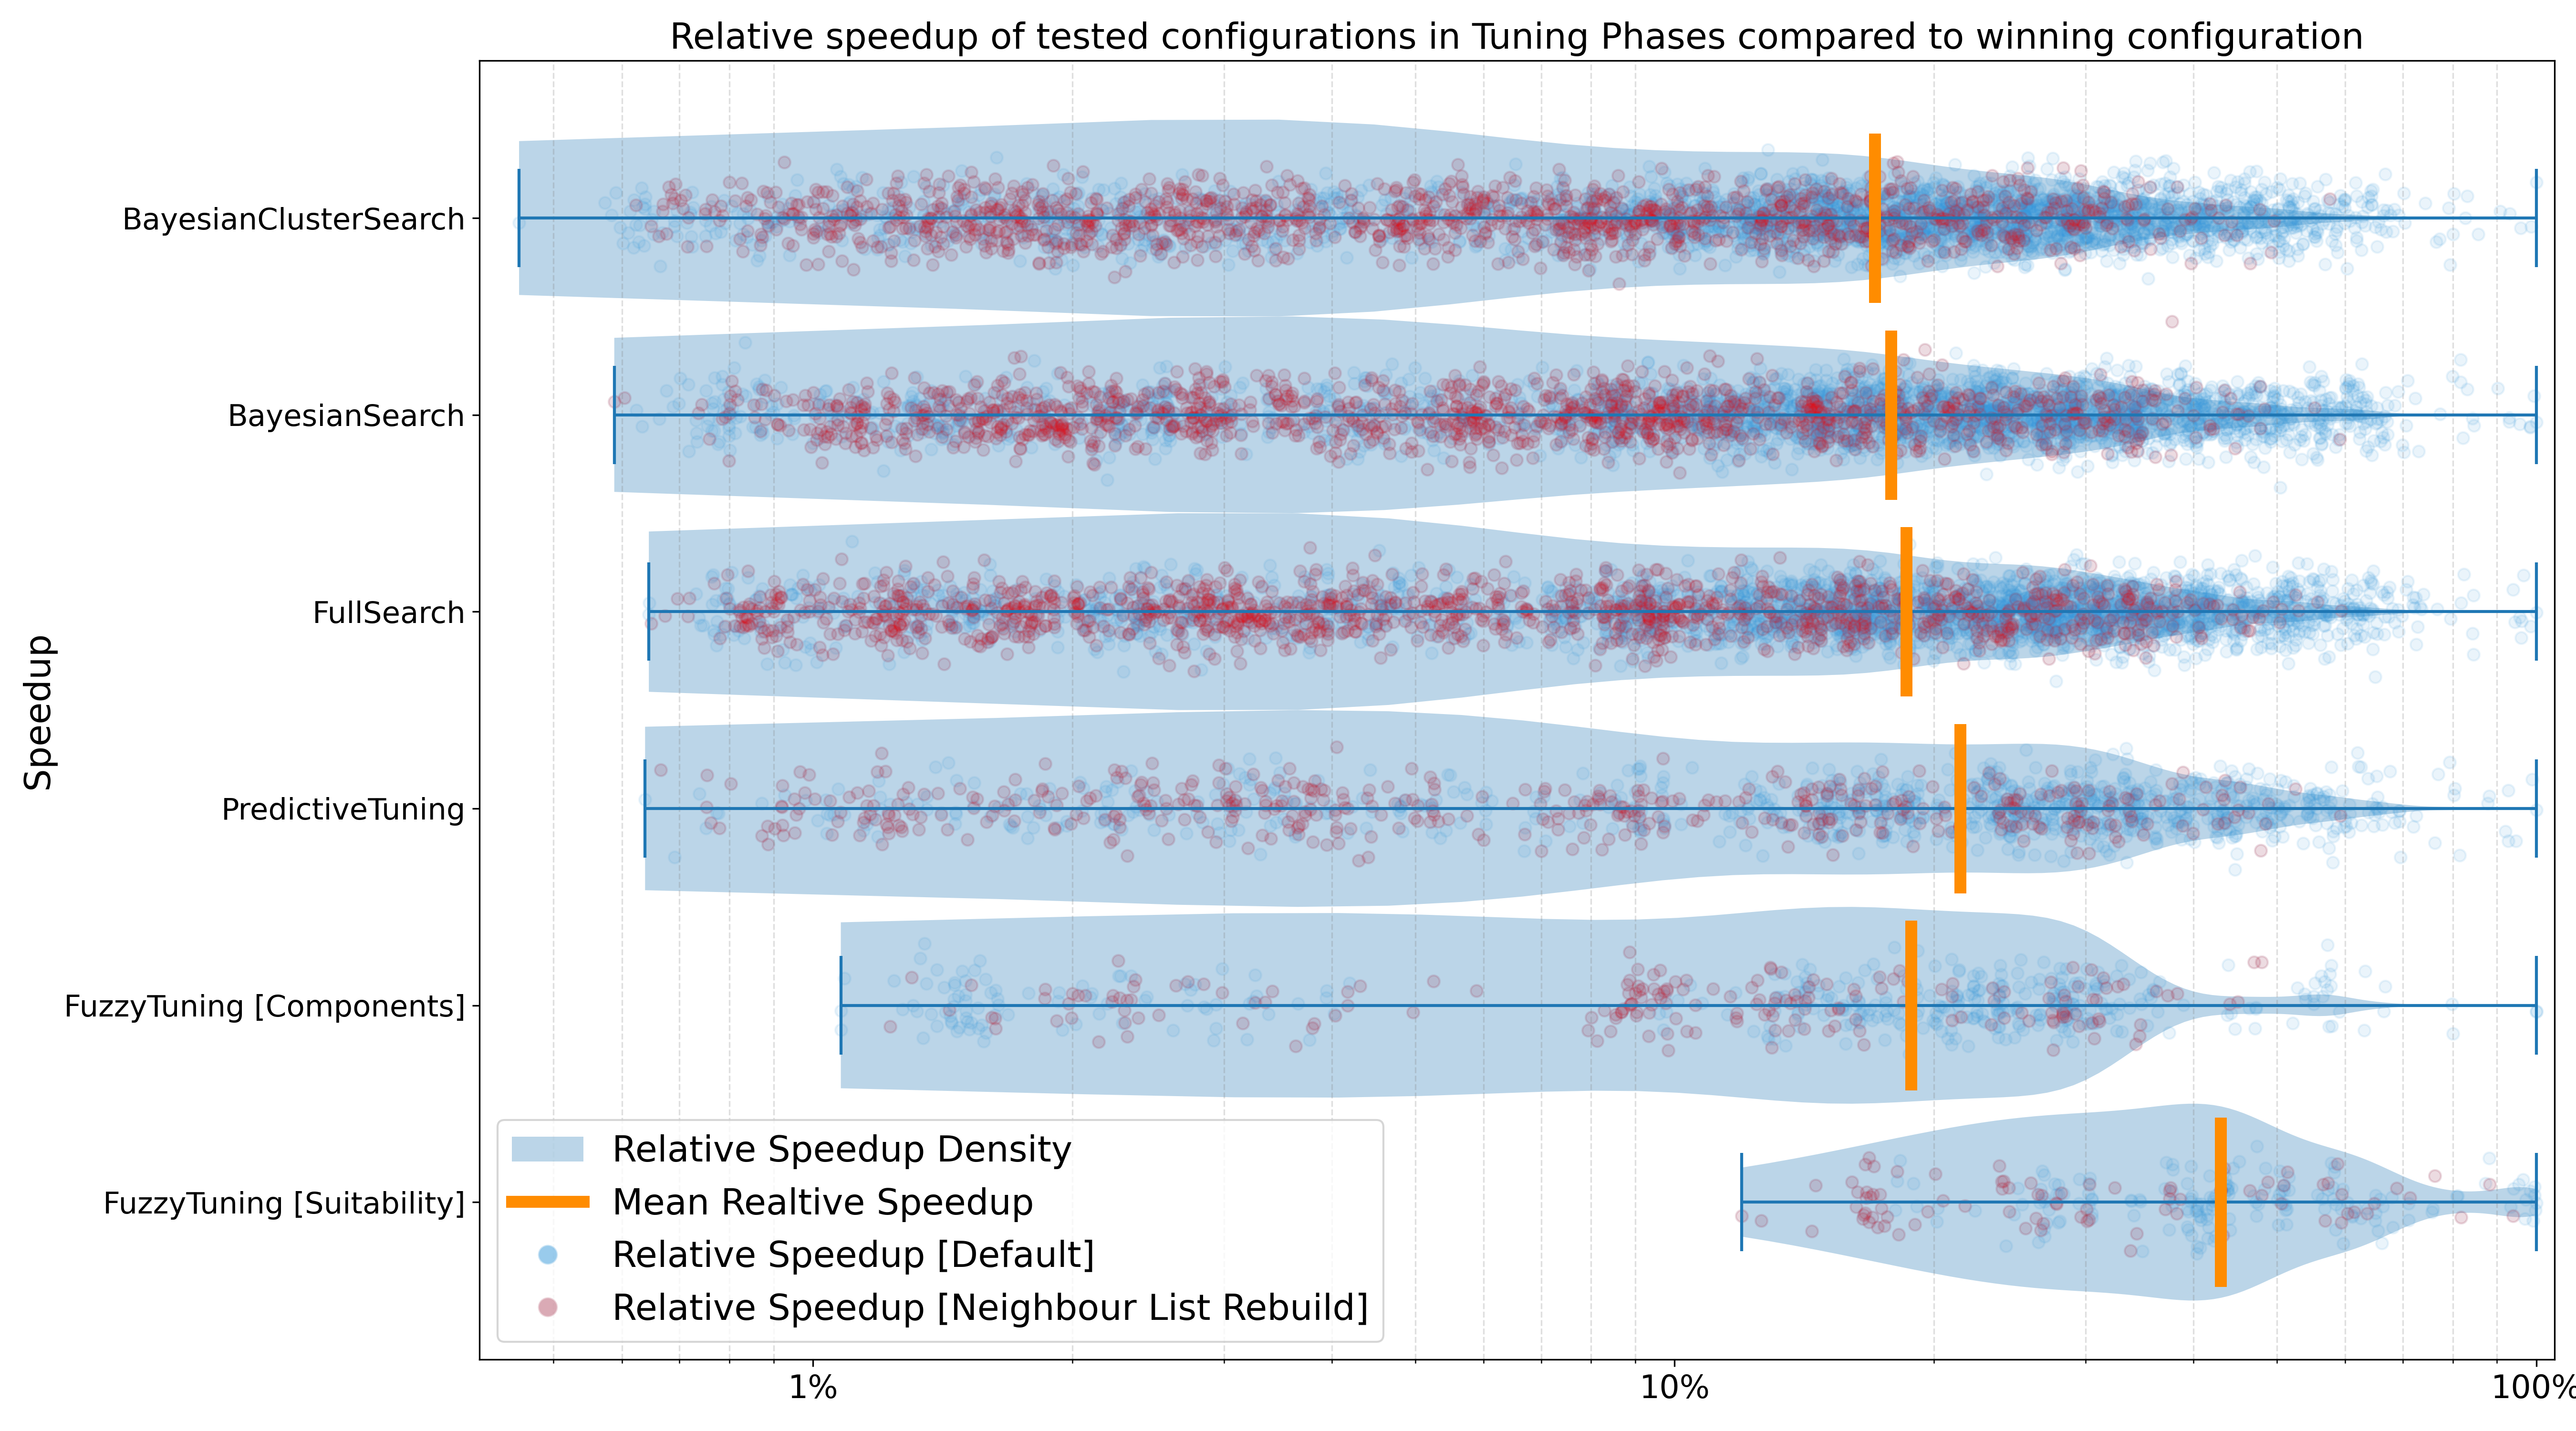
\includegraphics[width=\columnwidth,trim={1cm 0 0cm 1cm},clip]{figures/Benchmark/Observations/tuning_phase_speedup_SpinodalDecompositionMPI_14_0.png}
        \caption{Rank 0 of the Spinodal Decomposition MPI scenario with 14 threads.}
        \label{fig:spinodalSpeedupDensity}
    \end{subfigure}


    \caption[Quality of predictions during tuning phases]{The plot shows the speedup density distribution of all configurations evaluated during the tuning phases of both the Exploding Liquid and Spinodal Decomposition MPI scenarios calculated from the smoothed timings (see \autoref*{des:tuningdatafields}). The fuzzy tuning strategies generally encounter better configurations during the tuning phases, which improves their total performance.}
    \label{fig:tuningPhaseSpeedup}
\end{figure}


\begin{figure}
    \centering
    \includegraphics[width=\columnwidth]{figures/Benchmark/SuitabilitySearch/SuitabilityExploding_timings_threshold_benchmark-cluster_suitability-tuning-exploding_1.png}
    \caption[Exploding liquid benchmark with different suitability thresholds]{Exploding liquid benchmark with different suitability thresholds. The suitability threshold specifies the width of the interval around the best configuration, which determines how many configurations are selected for the tuning phase. Very low thresholds perform poorly, as they leave no margin for error and fail to select the best configuration. Very high thresholds also perform poorly, as high suitability values cause the strategy to behave like FullSeach. The optimal threshold for this scenario is between 20\% and 40\%.}
    \label{fig:suitabilityThreshold}
\end{figure}
\chapter{Future Work}
\label{sec:future_work}

In this chapter, we discuss some of the possible improvements that could be made to the current system to improve its performance and usability.

\section{Dynamic Rule Generation}

The current rule extraction process is static and requires a pre-collected dataset of selected scenarios. This is an obvious limitation, as users cannot be expected to collect a dataset of scenarios prior to using the library. Another issue is that the generated rules can only be expected to perform well in scenarios similar to the ones in the dataset, preventing the rules from being shared between vastly different use cases.

One could look into ways of adaptively updating the expert knowledge as new scenarios are encountered. This could be done by spending extra time during the simulation to evaluate the performance data of recently or additionally executed configurations and update the expert knowledge accordingly by retraining the underlying Decision Trees on the fly.

\section{Improving Tuning Strategies}

As previously discussed in \autoref{sec:earlyStopping}, all current tuning strategies suffer from evaluating extremely bad configurations during the tuning phases. Especially for strategies without rule-based selection, this is a significant issue and causes enormous tuning overhead that could be avoided. Implementing an early stopping mechanism could drastically improve all tuning strategies and thus benefit the core idea of AutoPas.

\section{Simplification of the Fuzzy System to Decision Trees}

As the current way of generating the Fuzzy Systems with the data-driven approach already makes use of Decision Trees, one could look into ways of directly using the Decision Trees to make decisions.

The currently used implementation of the Component Tuning approach, already is quite close to a Decision Tree approach as it used the MOM defuzzification. Since this aproach showed good results, it is possible that the Fuzzy Tuning approach could be simplified to a Decision Tree approach without losing much performance. This would make the tuning process more transparent and easier to understand for users, as the complexity intrpduced by fuzzy sets and membership functions could be avoided.

To test this hypothesis using the current system, one could change membership functions to crisp splits as originally depicted in \autoref{fig:fuzzyMembershipFunctions} and rerun the benchmarks to see if the performance is still comparable. Such a rule file would emulate (Crisp) Decision Trees, following the same rules but without the fuzziness.
\chapter{Conclusion}
\label{sec:conclusion}

This thesis introduced a novel fuzzy logic-based tuning strategy for AutoPas and implemented a generic Fuzzy Tuning Library into the AutoPas framework, providing a reusable foundation for future research projects.

\medskip

\noindent A key contribution was the development of a data-driven approach to automatically generate competitive fuzzy systems, enabling the tuning of complex systems without extensive prior knowledge. The results demonstrated that the proposed Fuzzy Tuning Strategy significantly outperformed existing tuning strategies on selected benchmarks, substantially reducing the total simulation runtime by up to a factor of 1.96.

\medskip

\noindent While the fuzzy tuning strategy and the data-driven rule generation process showed promise, they are not universal solutions, as considerable upfront effort is necessary to collect the data to generate the rule base. Since such a workload cannot be expected from typical users of AutoPas, future research is needed to streamline the data collection and rule generation process to make the fuzzy tuning strategy more accessible to a broader audience.

\medskip

\noindent In conclusion, the Fuzzy Tuning Strategy and the data-driven rule generation process represent a significant step forward in tuning AutoPas simulations and offer a solid foundation for future research. While challenges remain in making it more accessible and broadly applicable, the potential for substantial performance gains makes this an exciting area for continued investigation and refinement.

% -------------------------------------------------------------------------------
% ---------------------------------- APPENDIX -----------------------------------
% -------------------------------------------------------------------------------

\appendix

\chapter{Appendix}

\printglossaries

\newpage

\section{LiveInfoLogger Data Fields}
\label{des:liveinfodatafields}

The following fields are currently available in the LiveInfo data file, which contains information about the simulation state at each iteration. The data is collected and logged by the \texttt{LiveInfoLogger} class of the \gls{autopas} library.

\begin{description}[style=multiline, leftmargin =40mm]
    \item [Iteration] The current iteration number of the simulation.
    \item [avgParticlesPerCell] The average number of particles per cell in the simulation domain.
    \item [cutoff] The cutoff radius for the interaction of particles, beyond which particles do not interact.
    \item [domainSizeX] The size of the simulation domain in the X dimension.
    \item [domainSizeY] The size of the simulation domain in the Y dimension.
    \item [domainSizeZ] The size of the simulation domain in the Z dimension.
    \item [estimatedNumNeighborInteractions] The estimated number of neighbor interactions between particles.
    \item [homogeneity] A measure of the distribution uniformity of particles across the cells. \todo{Define the metric}
    \item [maxDensity] The maximum density of particles in any cell.
    \item [maxParticlesPerCell] The maximum number of particles found in any single cell.
    \item [minParticlesPerCell] The minimum number of particles found in any single cell.
    \item [numCells] The total number of cells in the simulation domain.
    \item [numEmptyCells] The number of cells that contain no particles.
    \item [numHaloParticles] The number of particles in the halo region (boundary region) of the simulation domain.
    \item [numParticles] The total number of particles in the simulation domain.
    \item [particleSize] The size of each particle. \todo{Which unit?}
    \item [particleSizeNeededByFunctor] The particle size required by the functor (the function used for calculating interactions).
    \item [particlesPerBlurredCellStdDev] The standard deviation of the number of particles per blurred cell, providing a measure of particle distribution variability.
    \item [particlesPerCellStdDev] The standard deviation of the number of particles per cell, indicating the variability in particle distribution.
    \item [rebuildFrequency] The frequency at which the neighbor list is rebuilt.
    \item [skin] The skin width added to the cutoff radius to create a buffer zone for neighbor lists, ensuring efficient interaction calculations.
    \item [threadCount] The number of threads used for parallel processing in the simulation.
\end{description}


\section{TuninData Fields}
\label{des:tuningdatafields}

The following fields are currently available in the TuningResults data file, which contains the current performance data for a given configuration at a particular iteration. The data is collected and logged by the \texttt{TuningDataLogger} class of the \gls{autopas} library.

\begin{description}[style=multiline, leftmargin =40mm]
    \item[Date] The date and time when the data was collected.
    \item[Iteration] The current iteration number of the simulation.
    \item[Container] The type of container used to store the particles in the simulation (e.g., LinkedCells, VerletLists).
    \item[CellSizeFactor] A factor that determines the size of the cells relative to the cutoff radius. \todo{check https://mediatum.ub.tum.de/doc/1518839/1518839.pdf}
    \item[Traversal] The method used to traverse the cells and calculate interactions between particles.
    \item[Load Estimator] The strategy used to estimate and balance the computational load across different parts of the simulation domain.
    \item[Data Layout] The arrangement of particle data in memory (e.g., AoS for Array of Structures, SoA for Structure of Arrays).
    \item[Newton 3] Indicates whether the Newton's third law optimization is used to reduce computation by only calculating forces once per particle pair (Yes/No).
    \item[sample$i$] The performance data for the configuration at the $i$-th sample point. The number of total sample points per iteration can be configured via the \texttt{.yaml} configuration file.
    \item[Reduced] The reduced performance data for all sample points, calculated by aggregating the data across all sample points. The specific aggregation method can be configured via the \texttt{.yaml} configuration file.
    \item[Smoothed] A smoothed version of the reduced performance data.

\end{description}


\section{ANTLR4 Rule Parser Grammar}

The following is the grammar for the domain-specific language used by the Rule Parser to parse the rule base supplied by the user. The grammar is defined using the ANTLR4 parser generator.


\lstset{
    backgroundcolor=\color{gray!10},
    framexleftmargin=5pt,
    framextopmargin=5pt,
    numbers=left,
}%

% Applies only when you use it
\lstdefinestyle{MyLang}{
    basicstyle=\small\ttfamily,%
    breaklines=true,%                                      
    moredelim=[s][\color{green!50!black}\ttfamily]{'}{'},
    commentstyle={\color{gray}\itshape},%                  
    morecomment=[l]{//},
    morekeywords={rule_file, settings, linguistic_variable, fuzzy_term, function, fuzzy_rule, fuzzy_set, output_mapping, output_entry, pattern_mapping, config_pattern},
    keywordstyle={\color{red!90!black!70}\bfseries},%
    emph={STRING, NUMBER, IDENTIFIER, WS, COMMENT, INT, EXP, EOF},
    emphstyle={\color{blue}\ttfamily},
}


\begin{lstlisting}[style=MyLang, caption={ANTLR4 Rule Parser Grammar}, label={lst:antlr4grammar}]
grammar FuzzyLanguage;

// Rule File
rule_file           : settings linguistic_variable* 
                      output_mapping fuzzy_rule* EOF
                    ;

// Settings as key-value pairs
settings            : 'FuzzySystemSettings' ':'
                    (IDENTIFIER ':' STRING)*
                    ;

// Fuzzy Variable
linguistic_variable
                    : 'FuzzyVariable' ':' 'domain' ':' STRING 
                        'range' ':' '(' NUMBER ',' NUMBER ')' 
                       fuzzy_term+
                    ;

fuzzy_term
                    : STRING ':' function
                    ;

function
                    : IDENTIFIER '(' NUMBER (',' NUMBER)* ')'
                    ;

// Fuzzy Rule
fuzzy_rule
                    : 'if' fuzzy_set 'then' fuzzy_set
                    ;

fuzzy_set
                    : '(' fuzzy_set ')'         # Brackets
                    | fuzzy_set '&&' fuzzy_set  # And
                    | fuzzy_set '||' fuzzy_set  # Or
                    | '!' fuzzy_set             # Negate
                    | STRING '==' STRING        # Select
                    ;

// Output Mapping
output_mapping
                    : 'OutputMapping' ':'
                       output_entry+
                    ;

output_entry
                    : STRING ':' pattern_mapping+
                    ;

pattern_mapping
                    : NUMBER '=>' 
                        config_pattern (',' config_pattern)*
                    ;

config_pattern
                    : '[' (IDENTIFIER '=' STRING) 
                          (',' IDENTIFIER '=' STRING)* ']'
                    ;

// Lexer Rules
WS
                    : [ \t\n\r\f]+ -> skip
                    ;

COMMENT             : '#' .*? '\r'? '\n' -> skip
                    ;

STRING
                    : '"' (~["\r\n] | '""')* '"'
                    {setText(getText().substr(1, getText().size()-2));}
                    ;

NUMBER
                    : '-'? INT ('.' [0-9]+)? EXP?
                    ;

fragment INT
                    : '0'
                    | [1-9] [0-9]*
                    ;

fragment EXP
                    : [Ee] [+-]? [0-9]+
                    ;

IDENTIFIER
                    : [a-zA-Z0-9_]+
                    ;
\end{lstlisting}

% -------------------------------------------------------------------------------
% ------------------------------ BIBLIOGRAPHY ------------------------------------
% -------------------------------------------------------------------------------

\listoffigures

\listoftables

\lstlistoflistings

\bibliographystyle{alpha}
\bibliography{literature}

\end{document}
